\documentclass{article}

\usepackage{amsmath}
\usepackage{amsfonts}
\usepackage{amssymb}
\usepackage{graphicx}
\usepackage{geometry}

\begin{document}
\title{Fringe Projection Simulator Manual}
\author{Tom Van Hoeydonck}
\date{February 24, 2002}
\maketitle
\part{Introduction}
\label{sec:Introduction}
Scanning three-dimensional objects has become a commonly used quality control procedure in the industry, but the techniques can still be improved.
To enhance the overall quality of the scans, scientists are looking for different measurement setups and more accurate algorithms.
Because building and aligning these setups is incredibly time-consuming, we developed software that simulates this method accurately. 
The software is capable of simulating the projection of fringes on complex models of over 400.000 vertices. The user can load the desired model 
as an stl-file, which is a supported file format in most regularly used CAD programs. The software can handle a projector with a diverging or 
telecentric lens. The calculated illumination pattern from the virtual projector is simulated on the complex object and all the gray values are 
calculated on a fragment base. The user can easily modify the frequency and the phase of the projection pattern so that spatial and temporal 
profilometry techniques can be simulated. To simulate Moir� measurements, a second grid can be oriented freely in space, for which the user 
can set the frequency and phase shift as well.
The virtual camera can also be operated with a diverging or telecentric lens. The above- mentioned options allow the operator to simulate both 
collimated and non-collimated projection and observation, with either parallel or crossed lens axes.
The software is available for 32-bit and 64-bit Windows operating systems and can be downloaded for free from our dedicated website:
http://www.fringesimulator.com (Now available at Github, licensed under the GPL license).
\begin{figure}
	\centering
	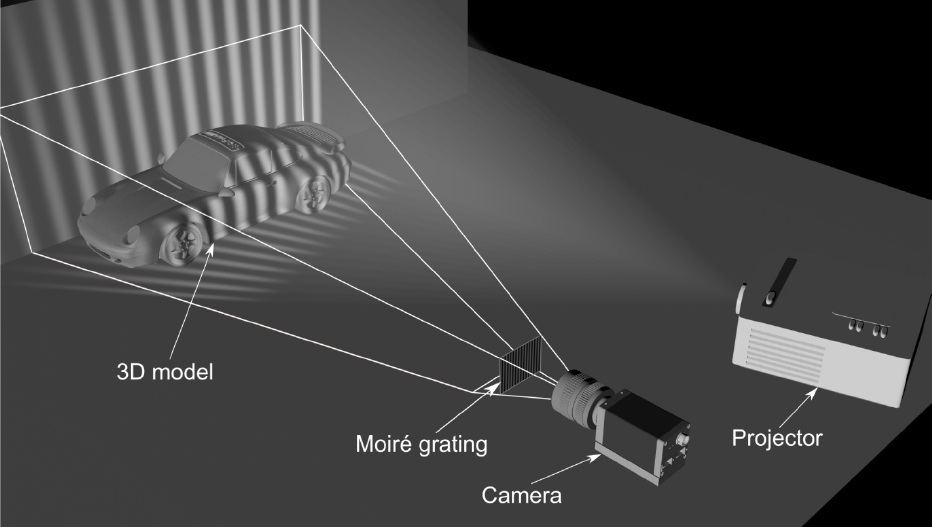
\includegraphics[width=0.90\textwidth, keepaspectratio=true]{Graphics/MoireGrating.jpg}
	\caption{Virtual projection Moir\'e profilometry setup (Moir\'e grating is multiplied with the camera image)}
	\label{fig:MoireGrating}
\end{figure}
\part{The Fringe Projection Simulator Screen}
\label{sec:TheFringeProjectionSimulatorScreen}
The program will start up after double-clicking the executable file : 'Fringe Projection Simulator 2012a.exe'.
The start up screen will look as shown in Figure \ref{fig:Startupscreen}.
\begin{figure}
	\centering
			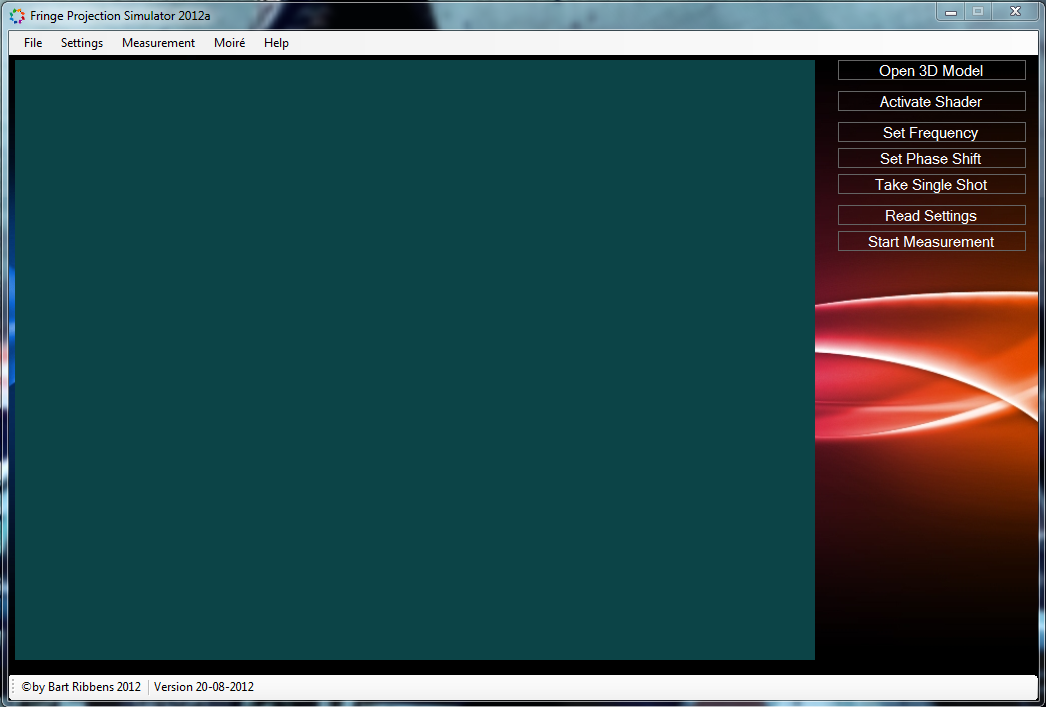
\includegraphics[width=1\textwidth, keepaspectratio=true]{Graphics/intro/Startupscreen.png}
	\caption{Fringe Projection Simulator screen}
	\label{fig:Startupscreen}
\end{figure}
The screen is divided into several areas, with each area having their own function.
Next Figure \ref{fig:StartupscreenWITHINFO} shows these different areas.
\begin{figure}
	\centering
			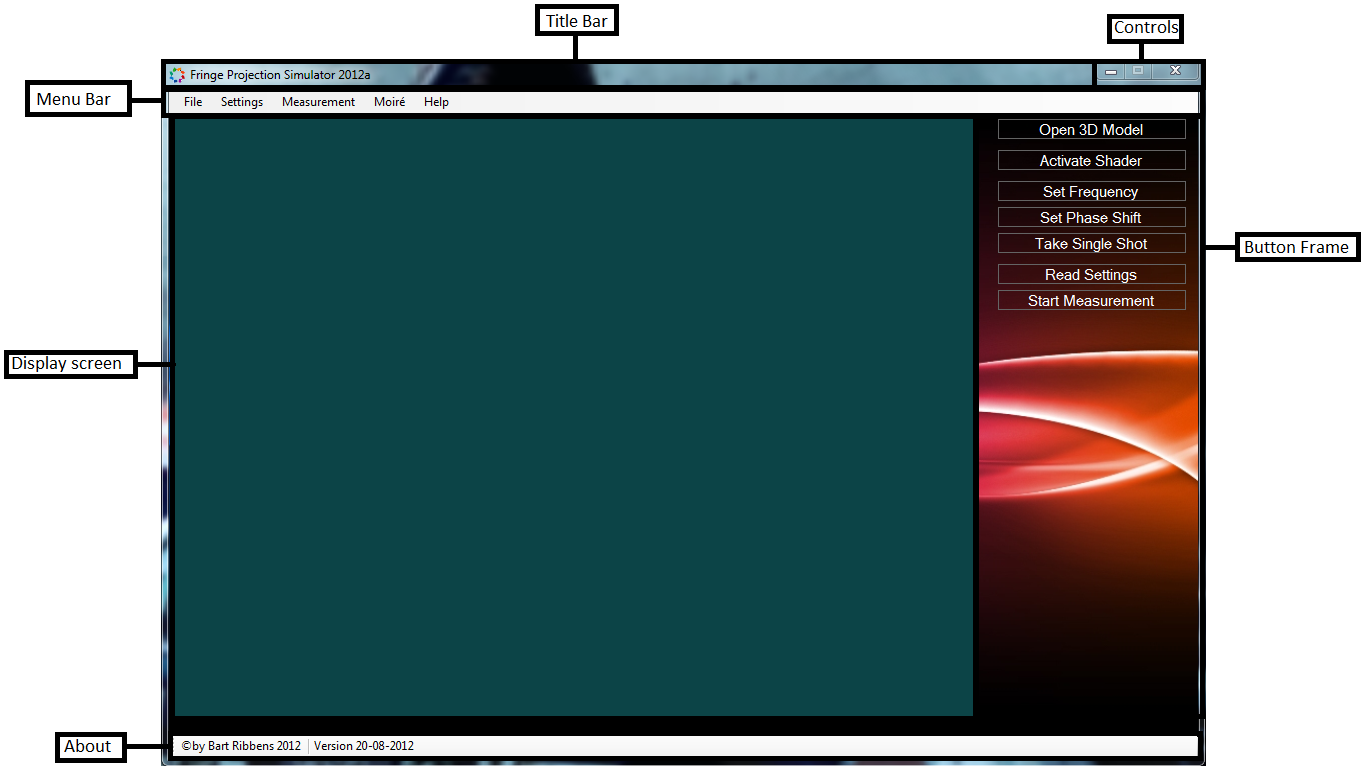
\includegraphics[width=1\textwidth, keepaspectratio=true]{Graphics/intro/StartupscreenWITHINFO.png}
			\caption{Startup screen}
	\label{fig:StartupscreenWITHINFO}
\end{figure}
\section{Title Bar}
\label{sec:TitleBar}
The title bar displays the title of the program that is running at the moment.
\section{The Menu Bar}
\label{sec:TheMenuBar}
The menu bar is used to navigate through the different controls within the program.
These different controls will be further explained in the next parts.
\section{Controls}
\label{sec:Controls}
The 3 controls buttons which are found in the top right corner, are used to hide or exit the program.
Maximizing or minimizing the program is not possible.
\section{Button Frame}
\label{sec:ButtonFrame}
This frame consists of several buttons, which are actually shortcuts to controls that can be found in the menu bar. 
Except for the read settings, this option is only available in the button frame.
\section{Display Screen}
\label{sec:DisplayScreen}
This screen will display our objects with the used shaders and gratings.
\section{About}
\label{sec:About}
This bar shows the creator of this program and the current version.
\part{The Fringe Simulation Controls}
\label{sec:TheFringeSimulationControls}
In this part we will explain all of the functions that are made possible with this program.
First, we have the buttons in the menu bar. These buttons are again divided into different buttons with different controls.
\section{File}
\label{sec:File}
When we click the file button in the menu bar, there will appear a pop up screen as shown in Figure \ref{fig:File}.
This means we have two controls we can execute within this menu.
\begin{figure}
	\centering
		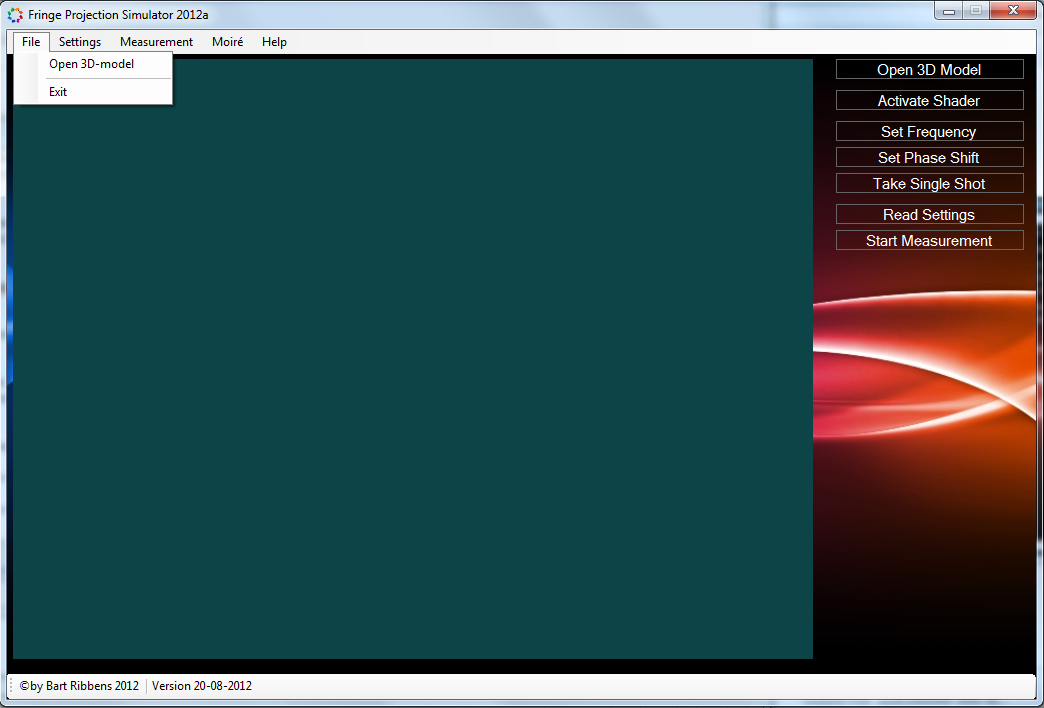
\includegraphics[width=0.75\textwidth, keepaspectratio=true]{Graphics/Beamer/File.png}
	\caption{File}
	\label{fig:File}
\end{figure}
\subsection{Open 3-D Model}
\label{sec:Open3DModel}
With this button, we can load a 3D Model within our program. The file has to be of the .STL extension, which means it consists of solely edges. The 3D model contains no volume.
Note that it is possible to create your own 3D Model with inventor and save it as an .STL file, this 3D model can be used in this program.
\subsection{Exit}
\label{sec:Exit}
When you click this button, the program will close.
\section{Settings}
\label{sec:Settings}
The next button in the menu bar, is the settings button. Figure
\ref{fig:settings} shows us which controls are accessible through this button.
\begin{figure}
	\centering
	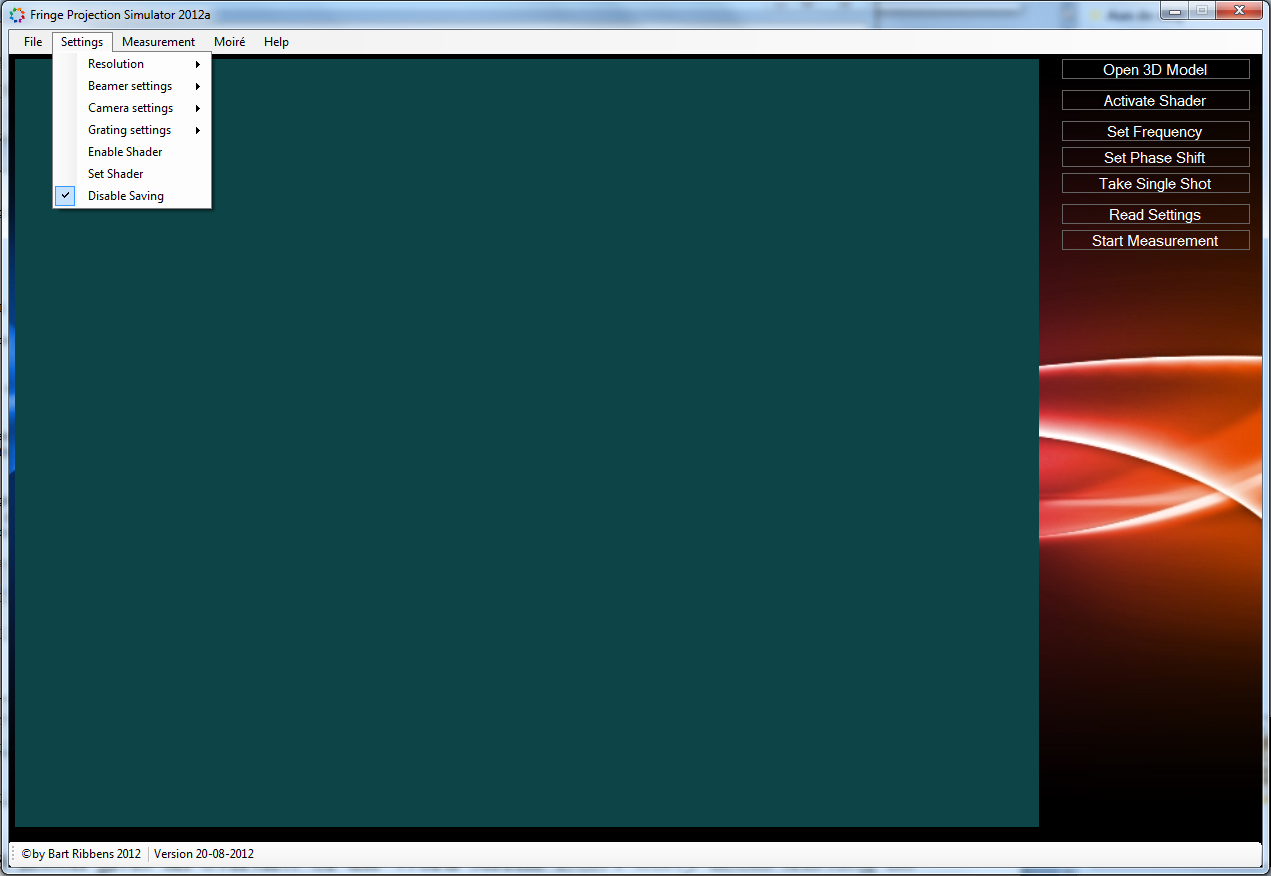
\includegraphics[width=1\textwidth, keepaspectratio=true]{Graphics/beamer/settings.png}
	\caption{Settings}
	\label{fig:settings}
\end{figure}
With these controls we can choose between different settings to change the setup of the simulation and manage the shaders.
\subsection{Resolution}
\label{sec:Resolution}
\begin{figure}
	\centering
		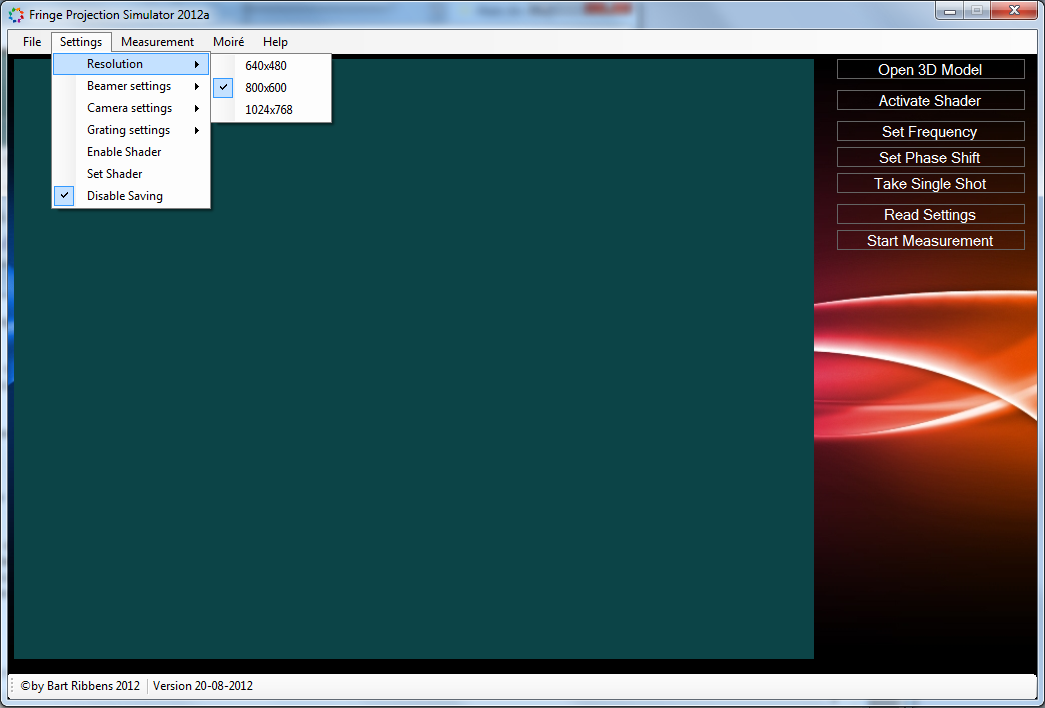
\includegraphics[width=1\textwidth, keepaspectratio=true]{Graphics/beamer/resolution.png}
	\caption{Resolution}
	\label{fig:resolution}
\end{figure}
Using the resolution button, we can change the display of our program. 
Standard we have a resolution of 800x600 pixels, this means that our program screen is 800 pixels in width and 600 pixels in height.
It is possible to change the resolution to other standard resolutions, such as : 640x480 or 1024x768.
Resolution 640x480 gives a smaller screen where the 1024x768 resolution results in a bigger screen.
\subsection{Beamer settings}
\label{sec:BeamerSettings}
\begin{figure}
	\centering
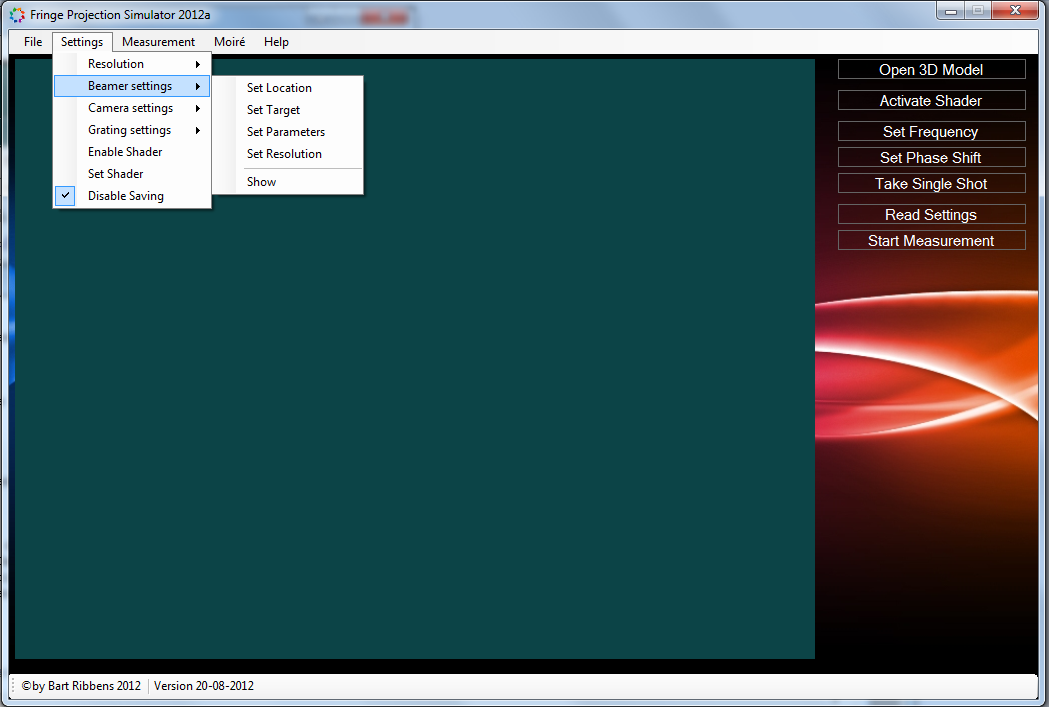
\includegraphics[width=0.75\textwidth, keepaspectratio=true]{Graphics/beamer/beamersettings.png}
	\caption{Beamer settings}
	\label{fig:beamer settings}
\end{figure}
This button allows us to change several properties of the beamer within the simulation.
\subsubsection{Set Location Beamer}
\label{sec:SetLocationBeamer}
Using the Set Location control, we can choose at which location our beamer is placed.
First, we have to enter an X value.
\begin{figure}
	\centering
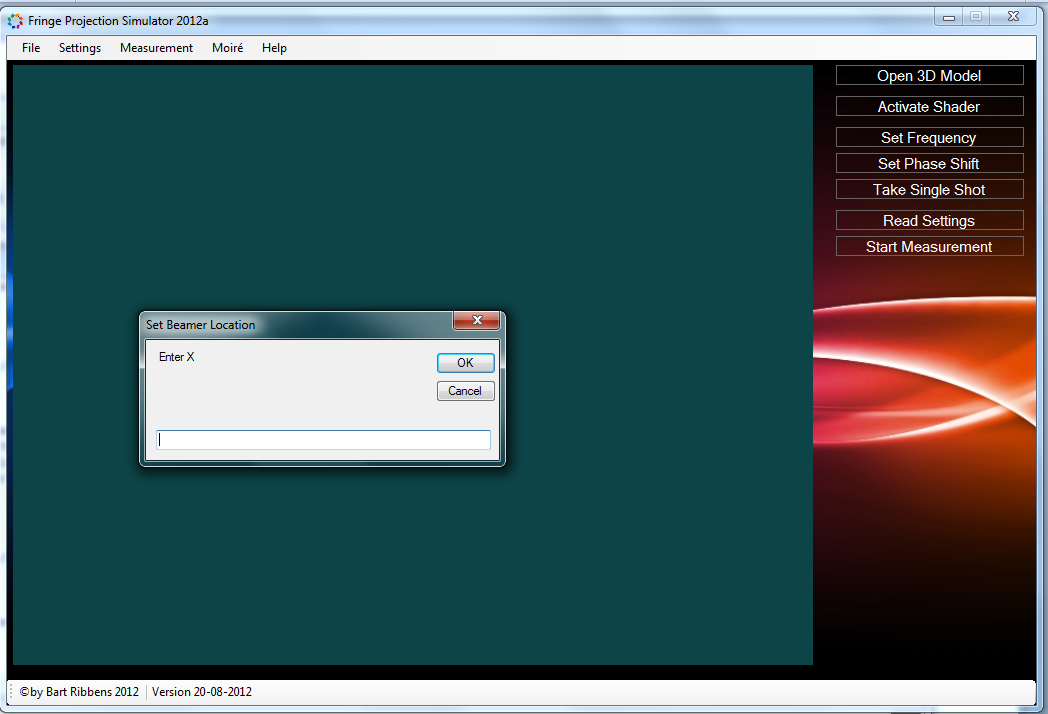
\includegraphics[width=1\textwidth, keepaspectratio=true]{Graphics/beamer/xlocationbeamer.png}
	\caption{X Beamer}
	\label{fig:xlocationbeamer}
\end{figure}
Next, is the Y value of the beamer.
\begin{figure}
	\centering
				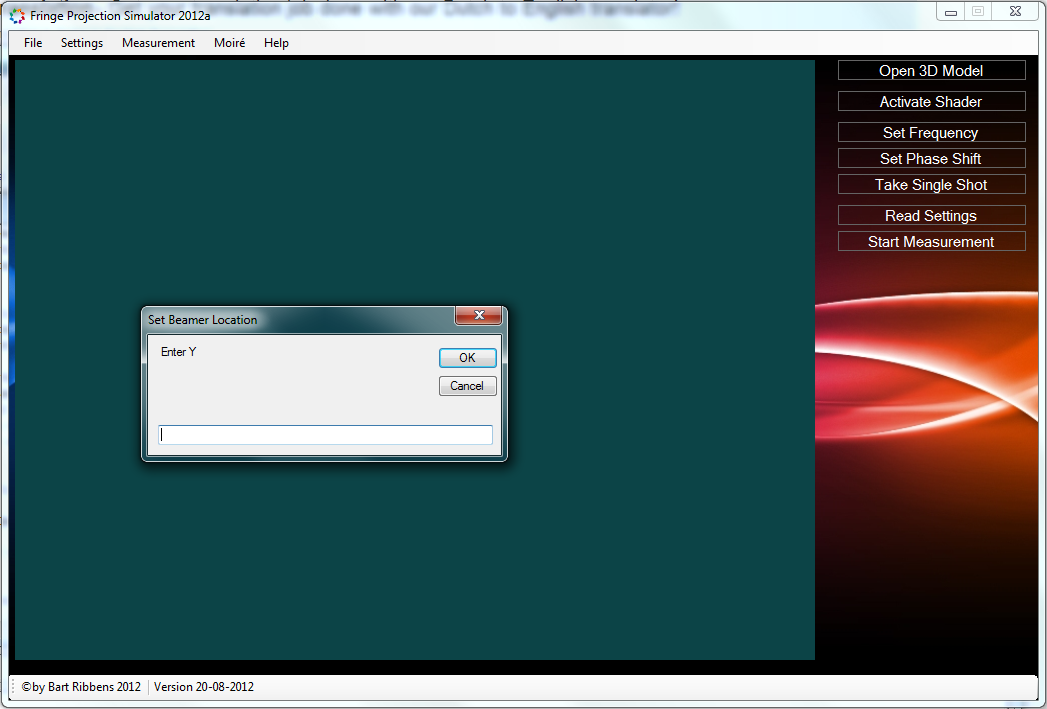
\includegraphics[width=1\textwidth, keepaspectratio=true]{Graphics/beamer/ylocationbeamer.png}
	\caption{Y Beamer}
	\label{fig:ylocationbeamer}
\end{figure}
Lastly, we have to fill in a Z value.
When this is done, we have given a location in space to the beamer.
\subsubsection{Set Target Beamer}
\label{sec:SetTargetBeamer}
With the Set Target control, we can choose at which position in space the beamer will be focused.
For example when the target has the coordinates (x = 10; y = 4; z = 2), the beamer will focus directly at that point.
\subsubsection{Set Parameters Beamer}
\label{sec:SetParametersBeamer}
We are able to adjust the parameters of the beamer with this control. 
The parameters consist of the beamer angle and the width/height ratio.
\begin{figure}
	\centering
	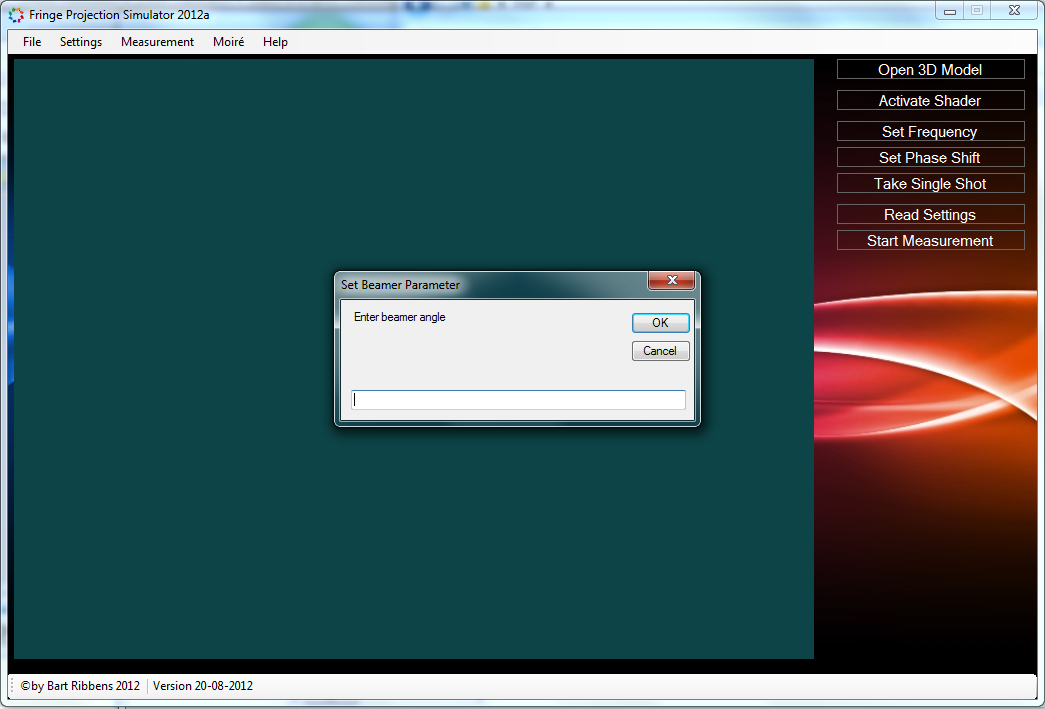
\includegraphics[width=1\textwidth, keepaspectratio=true]{Graphics/beamer/beamerangle.png}
	\caption{Beamer Angle}
	\label{fig:beamerangle}
\end{figure}
\paragraph{FOV (Field Of View)}
\label{sec:FOVFieldOfView}
First we enter the angle of the beamer, this is the same as the field of view.
The FOV (field of view) tells us how big the angle of our sight is. 
A FOV of 90 degrees gives us a larger sight than a FOV of 50 degrees.
The FOV gives us more information about how big our horizontal view is.
In \ref{fig:fov} we can easily see the difference between a FOV of 60 degrees on top and below a FOV of 90 degrees.
\begin{figure}
\centering
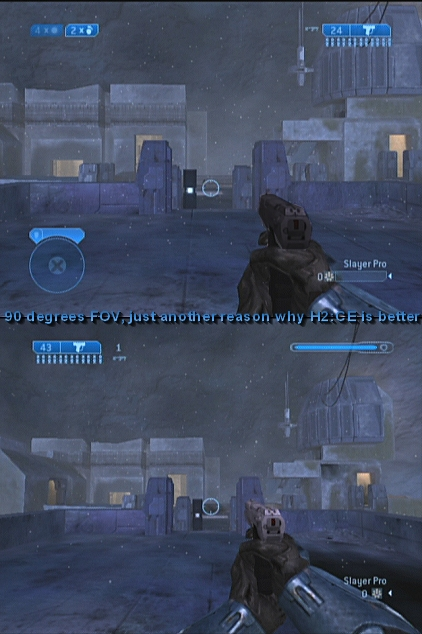
\includegraphics[width=0.85\textwidth, keepaspectratio=true]{Graphics/beamer/fov.png}
\caption{Field of view}
\label{fig:fov}
\end{figure}
\paragraph{Aspect Ratio}
\label{sec:AspectRatio}
Next, we are able to adjust the width/height ratio which we can use to determine the vertical view.
If we know the width of our beamer, we can easily determine the value of the height.
First we insert the aspect ratio, then we enter the width.
The standard used aspect ratio is 1,33. Figure
\ref{fig:ratio} shows us an example of a 2/1 aspect ratio.
\begin{figure}
	\centering
				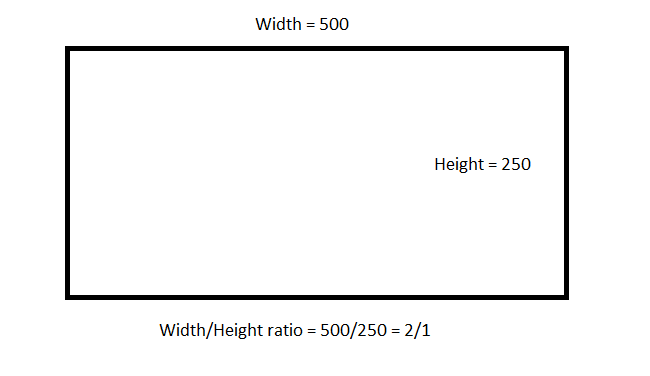
\includegraphics[width=0.85\textwidth, keepaspectratio=true]{Graphics/beamer/ratio.png}
	\caption{Ratio}
	\label{fig:ratio}
\end{figure}
\subsubsection{Set Resolution}
\label{sec:SetResolution}
We can set the resolution to a value which we prefer. It is advisable to choose a resolution, where there are no pixellations and other optic imperfections due to a low resolution.
An example of these imperfections is shown in Figure \ref{fig:image001}.
\begin{figure}
	\centering
				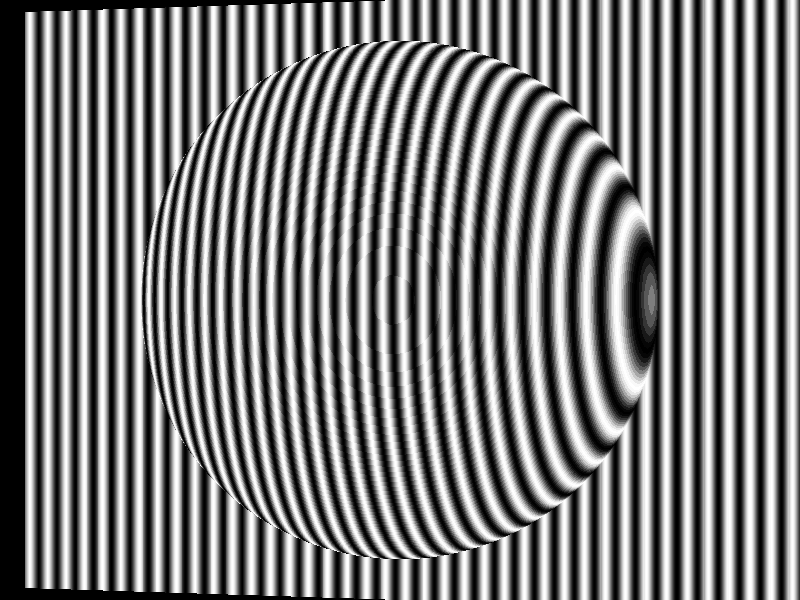
\includegraphics[width=0.85\textwidth, keepaspectratio=true]{Graphics/beamer/image001.png}
	\caption{Imperfections in image}
	\label{fig:image001}
\end{figure}
If you change the resolution to 1200x1200, there are clearly imperfections within the model. That is the reason why the resolution is standard set on 20000x20000, so that we certainly have a clear image.
\subsubsection{Show}
\label{sec:Show}
By clicking the show option, a pop up screen will appear which contains all the information about the beamer.
\begin{figure}
	\centering
				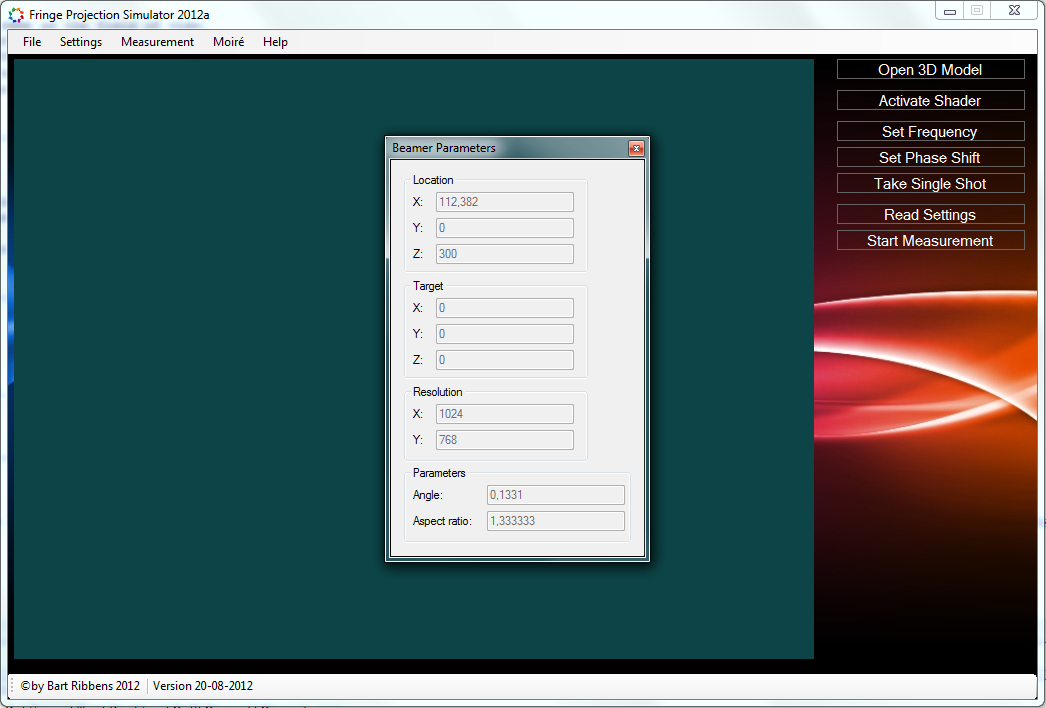
\includegraphics[width=0.85\textwidth, keepaspectratio=true]{Graphics/beamer/showbeamersettings.png}
				\caption{Show beamer settings}
	\label{fig:showbeamersettings}
\end{figure}
\subsection{Camera settings}
\label{sec:CameraSettings}
This control is used to change all the properties of the camera used in the simulation.
\begin{figure}
	\centering
		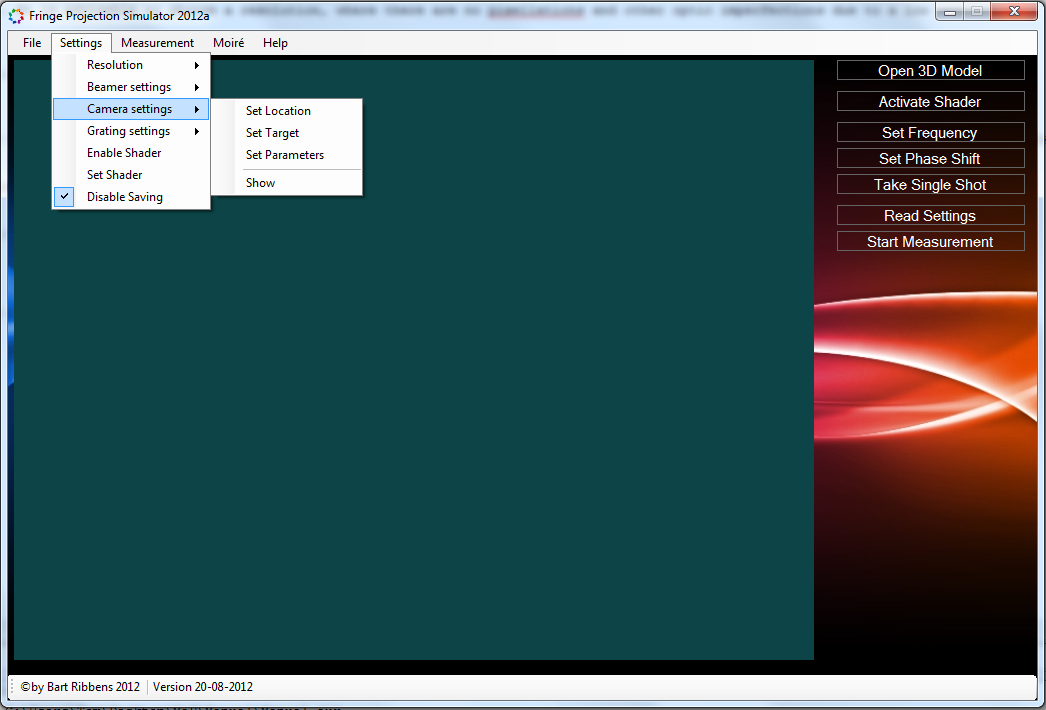
\includegraphics[width=0.85\textwidth, keepaspectratio=true]{Graphics/camera/camerasettings.png}
	\caption{Camera settings}
	\label{fig:camerasettings}
\end{figure}
\subsubsection{Set Location Camera}
\label{sec:SetLocationCamera}
Using the Set Location control, we can choose at which location our camera is placed.
First, we have to enter an X value.
\begin{figure}
	\centering
			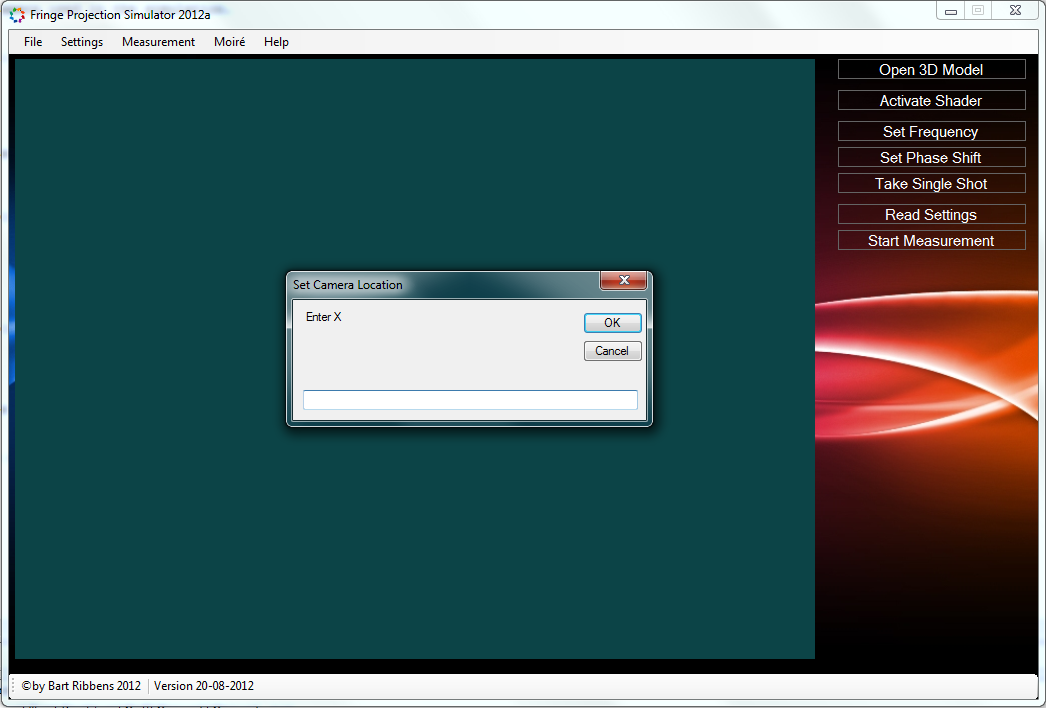
\includegraphics[width=0.85\textwidth, keepaspectratio=true]{Graphics/camera/xlocationcamera.png}
	\caption{X Beamer}
	\label{fig:xlocationbeamer}
\end{figure}
Next, is the Y value of the camera.
\begin{figure}
	\centering
					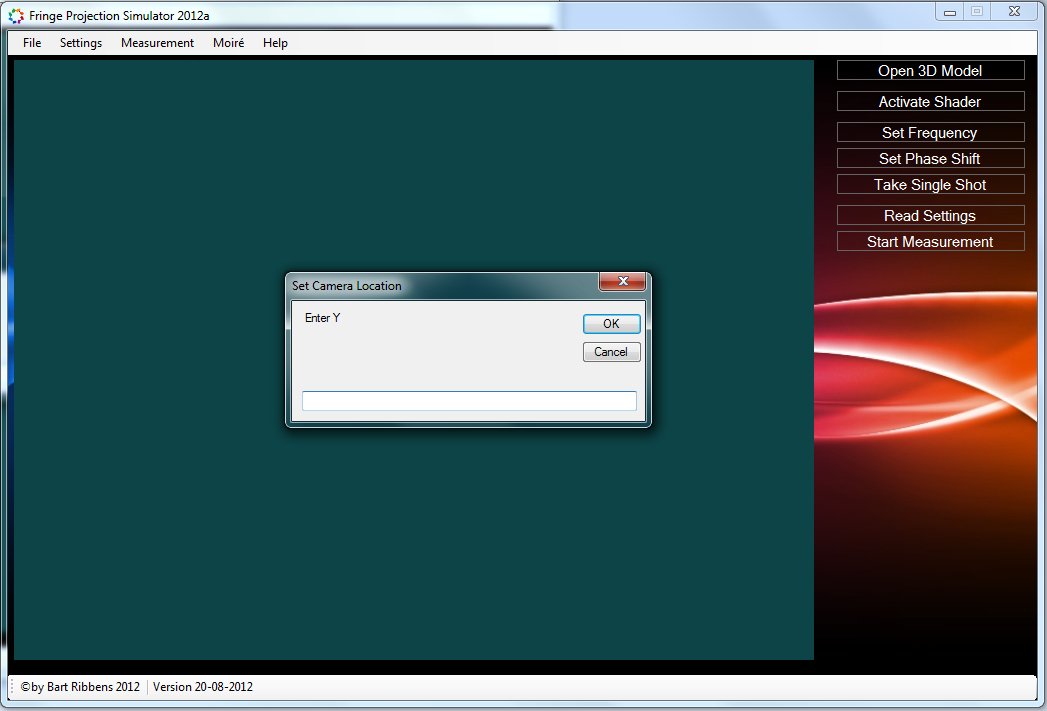
\includegraphics[width=0.85\textwidth, keepaspectratio=true]{Graphics/camera/ylocationcamera.png}
	\caption{Y Beamer}
	\label{fig:ylocationbeamer}
\end{figure}
Lastly, we have to fill in a Z value.
When this is done, we have given a location in space to the camera.
\subsubsection{Set Target Camera}
\label{sec:SetTargetCamera}
With the Set Target control, we can choose at which position in space the camera will be focused.
For example when the target has the coordinates (x = 10; y = 4; z = 2), the camera will focus directly at that point.
\subsubsection{Set Parameters Camera}
\label{sec:SetParametersCamera}
We are able to adjust the parameters of the camera with this control.
\paragraph{FOV}
\label{sec:FOV}
First, we can choose the FOV of the camera (which is explained in section \ref{sec:SetParametersBeamer}.
The FOV has to be within range 0-3,1.
\begin{figure}
	\centering
					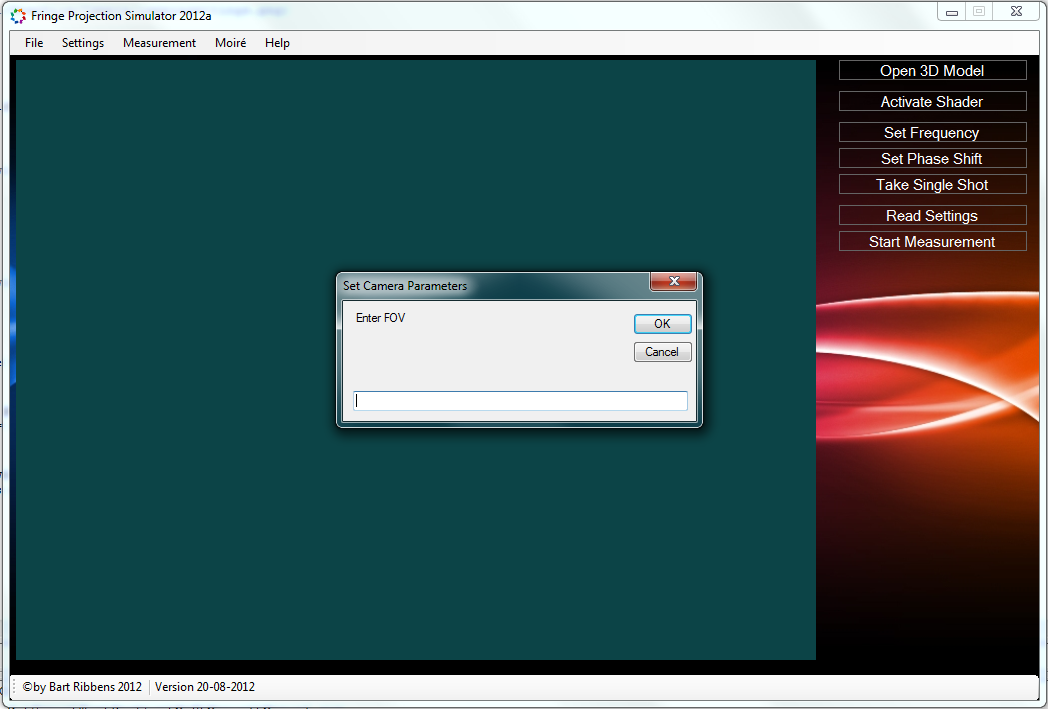
\includegraphics[width=0.85\textwidth, keepaspectratio=true]{Graphics/camera/camerafov.png}
	\caption{Camera FOV}
	\label{fig:camerafov}
\end{figure}
\paragraph{Aspect Ratio Camera}
\label{sec:AspectRatioCamera}
Next we are able to adjust the width/height ratio. The standard used aspect ratio is 1,33.
\begin{figure}
	\centering
					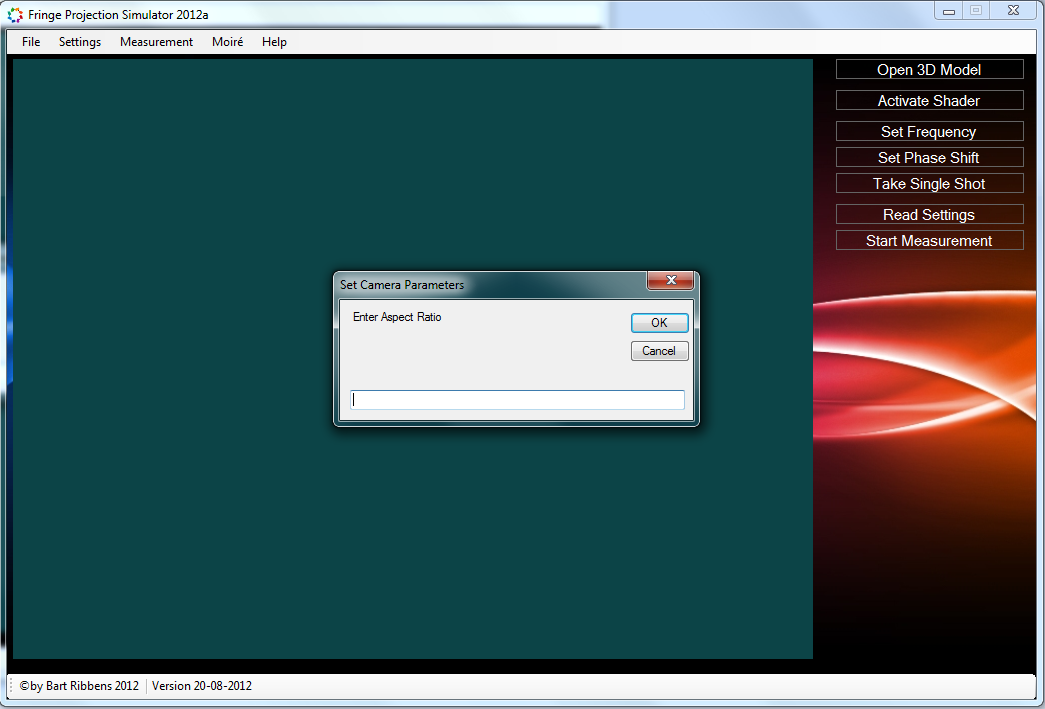
\includegraphics[width=0.85\textwidth, keepaspectratio=true]{Graphics/camera/aspectratiocamera.png}
	\caption{Aspect Ratio Camera}
	\label{fig:aspectratiocamera}
\end{figure}
\paragraph{Near Plane}
\label{sec:NearPlane}
The near plane is a distance from the camera, in which objects in front of this point, are not seen.
\begin{figure}
	\centering
					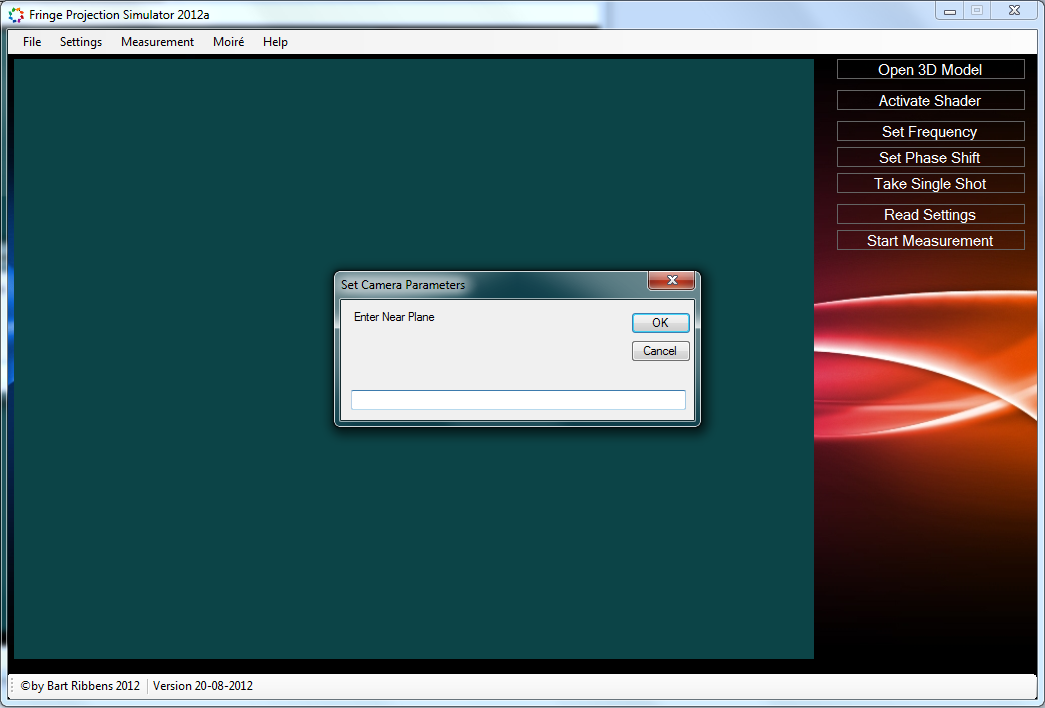
\includegraphics[width=0.85\textwidth, keepaspectratio=true]{Graphics/camera/nearplane.png}
	\caption{Near Plane}
	\label{fig:nearplane}
\end{figure}
\paragraph{Far Plane}
\label{sec:FarPlane}
This is the opposite of near plane, objects in front of this point are seen (except if they are also in front of the near plane).
Objects further then the far plane point, are not seen by the camera because they are too far away.
\begin{figure}
	\centering
					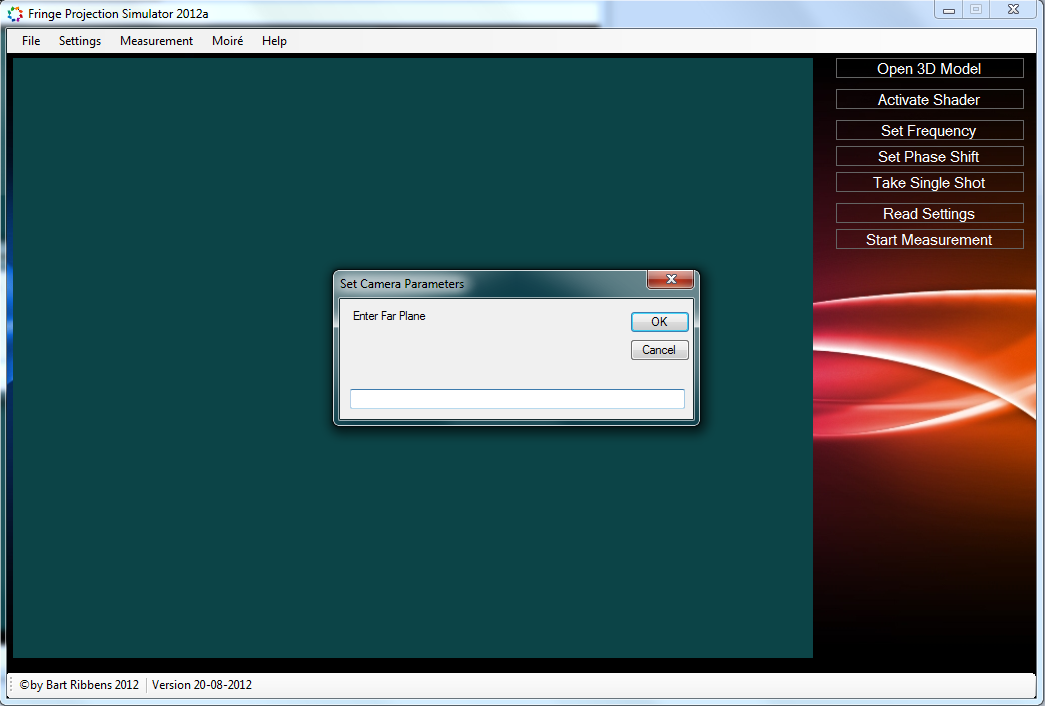
\includegraphics[width=0.85\textwidth, keepaspectratio=true]{Graphics/camera/farplane.png}
	\caption{Far Plane}
	\label{fig:farplane}
\end{figure}
\subsubsection{Show}
\label{sec:Show}
This control shows us all the properties of our camera.
\begin{figure}
	\centering
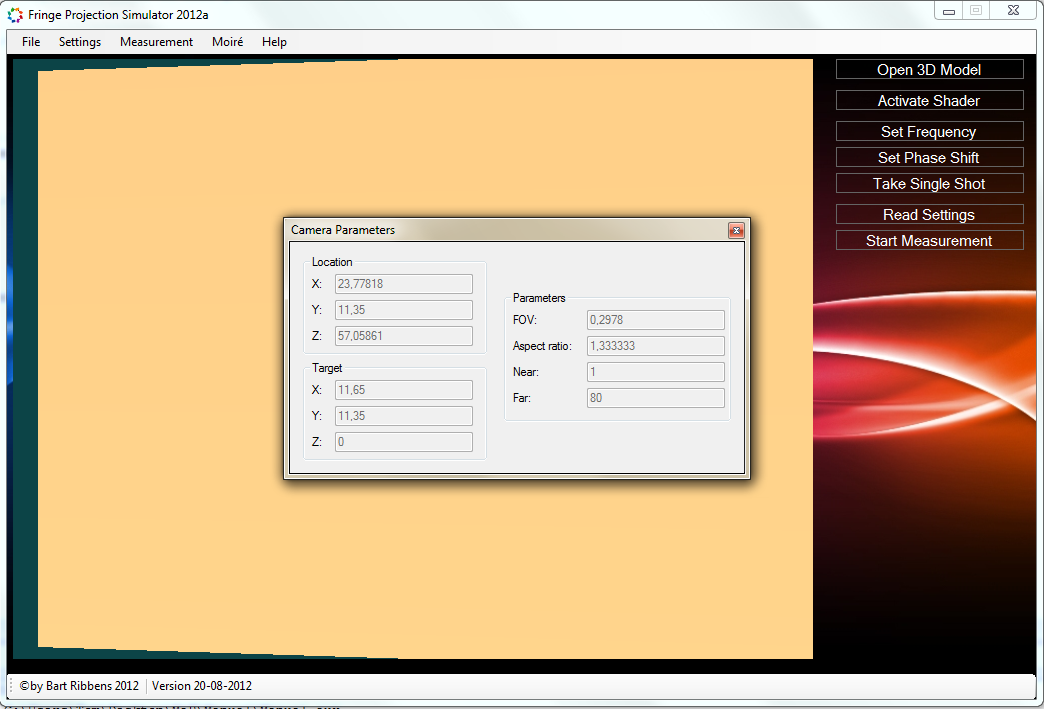
\includegraphics[width=1\textwidth, keepaspectratio=true]{Graphics/camera/showsettingscamera.png}	
					\caption{Settings Camera}
	\label{fig:showsettingscamera}
\end{figure}
\subsection{Grating Settings}
\label{sec:GratingSettings}
This button contains the settings of the grating used within the simulation.
\begin{figure}
	\centering
				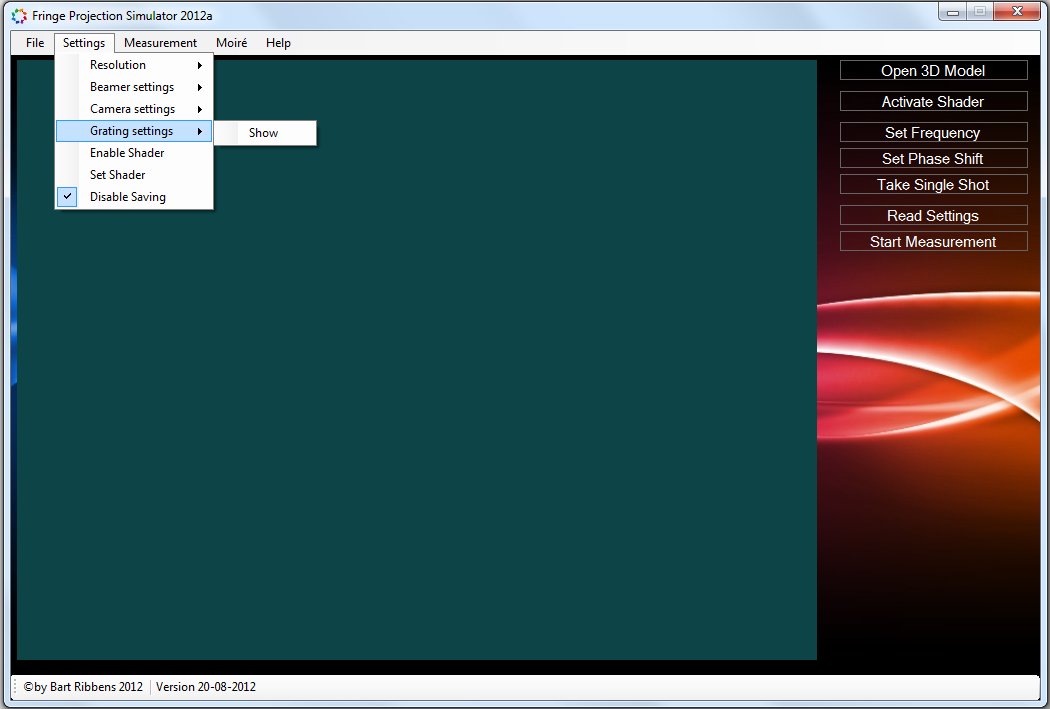
\includegraphics[width=0.85\textwidth, keepaspectratio=true]{Graphics/Grating/grating.png}
	\caption{Grating Settings}
	\label{fig:grating}
\end{figure}
\subsubsection{Show}
\label{sec:Show}
Clicking this button shows us all the properties of the grating.
\begin{figure}
	\centering
					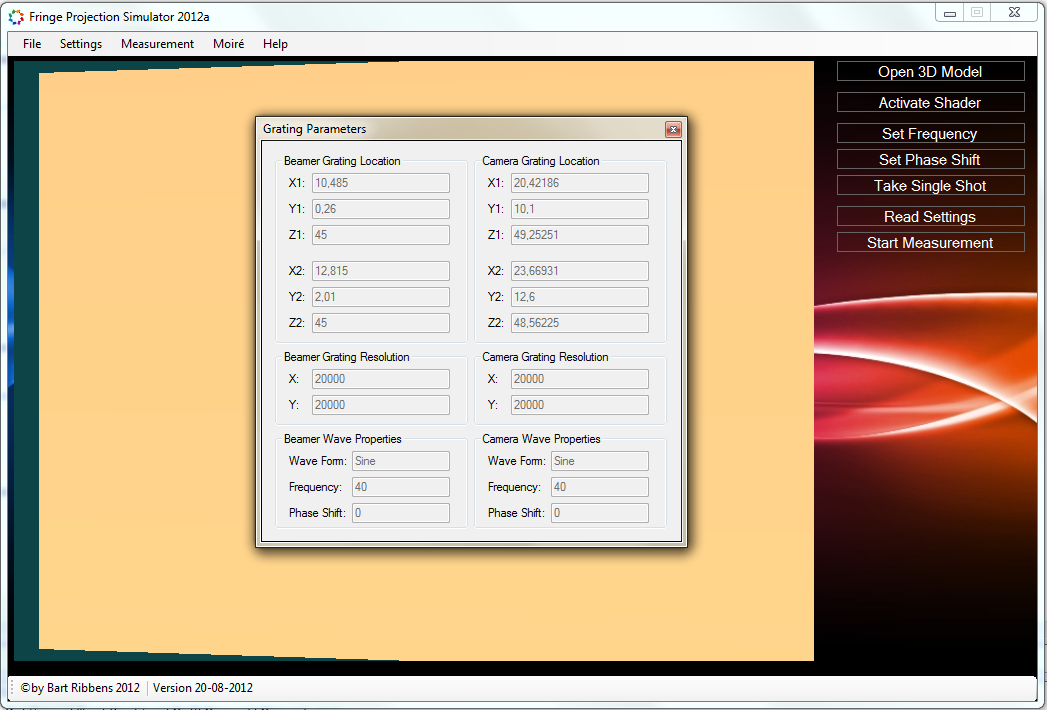
\includegraphics[width=0.85\textwidth, keepaspectratio=true]{Graphics/Grating/showgratingsettings.png}
	\caption{Show Grating Settings}
	\label{fig:showgratingsettings}
\end{figure}
\section{Enable Shader}
\label{sec:EnableShader}
By clicking the enable shader button, we can activate the beamer.
\begin{figure}
	\centering
					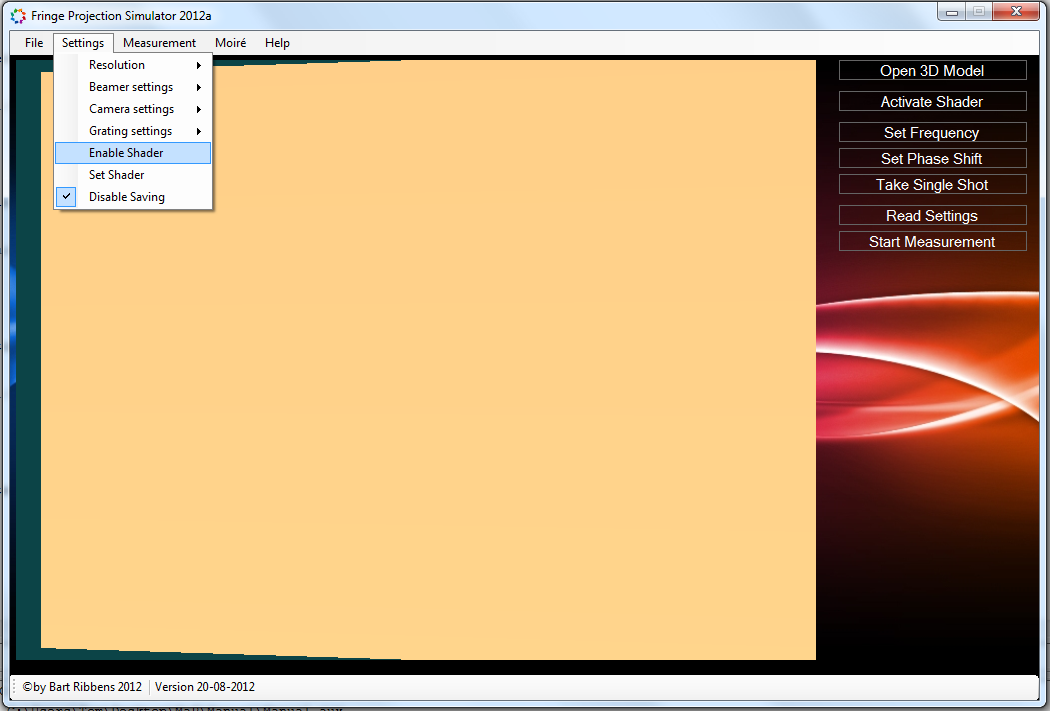
\includegraphics[width=0.85\textwidth, keepaspectratio=true]{Graphics/EnableDisableShader/enableshader.png}
	\caption{Enable Shader}
	\label{fig:enableshader}
\end{figure}
After we have enabled the shader, our display will look like Figure \ref{fig:shaderenabled}.
\begin{figure}
	\centering
	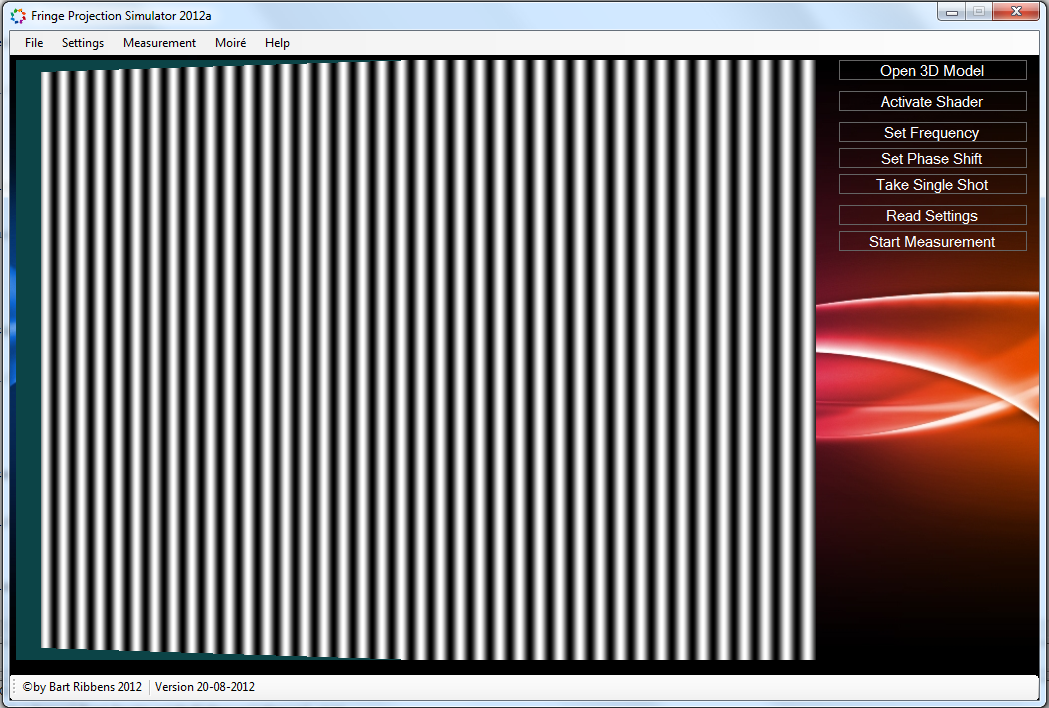
\includegraphics[width=0.85\textwidth, keepaspectratio=true]
	{Graphics/EnableDisableShader/shaderenabled.png}
	\caption{Shader Enabled}
	\label{fig:shaderenabled}
\end{figure}
We see a pattern that is projected onto our reference.
If we want to disable the shader, simply press on disable shader.
\begin{figure}
	\centering			
		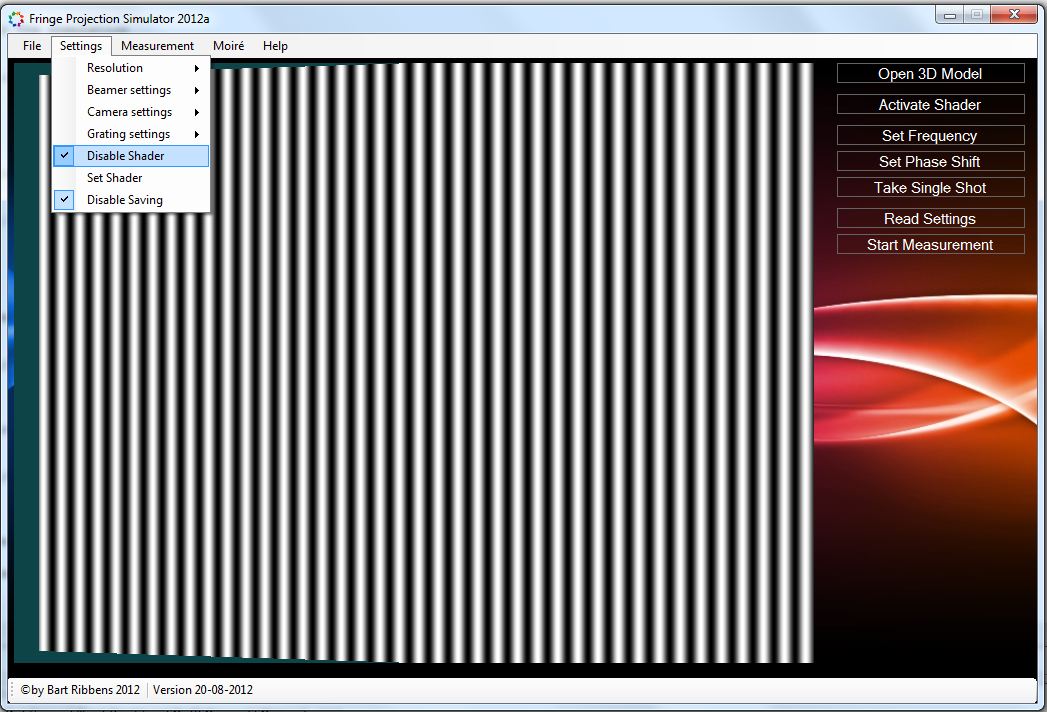
\includegraphics[width=0.85\textwidth, keepaspectratio=true]
	{Graphics/EnableDisableShader/disableshader.png}
	\caption{Disable Shader}
	\label{fig:disableshader}
\end{figure}
The pattern will disappear because we inactivated the shader.
\begin{figure}
	\centering
			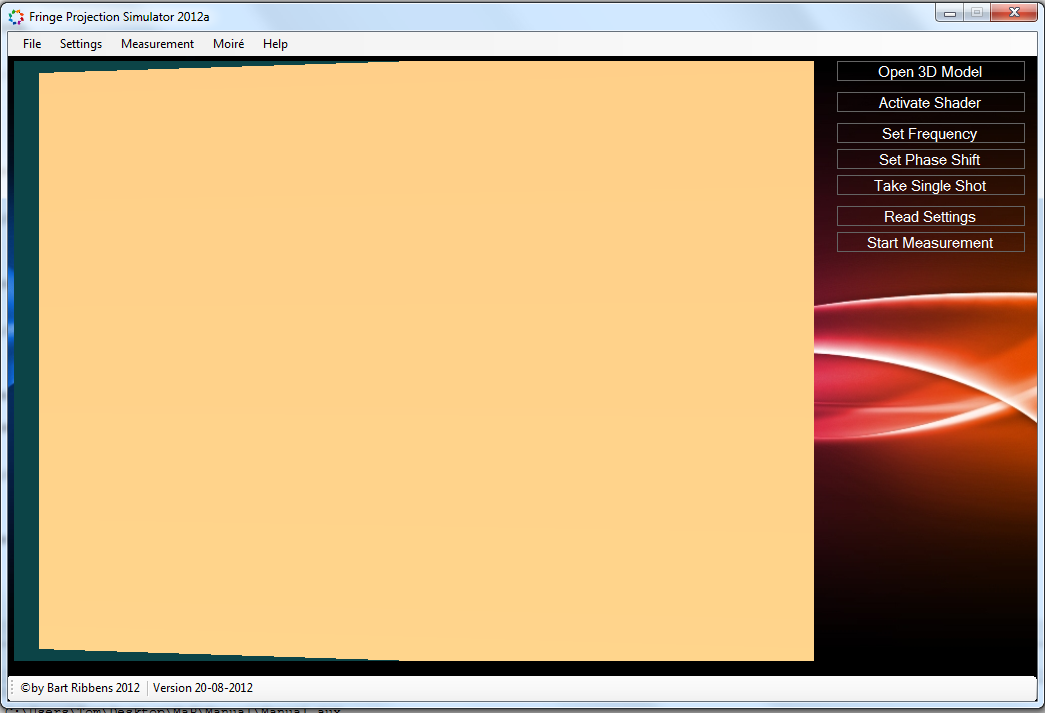
\includegraphics[width=0.85\textwidth, keepaspectratio=true]
	{Graphics/EnableDisableShader/inactiveshader.png}
	\caption{Shader Inactive}
	\label{fig:inactiveshader}
\end{figure}
\subsection{Set Shader}
\label{sec:SetShader}
The shaders used within this simulation are already loaded when the program is started.
If the user wants to load them manually, it can be done using this button.
\begin{figure}
	\centering
		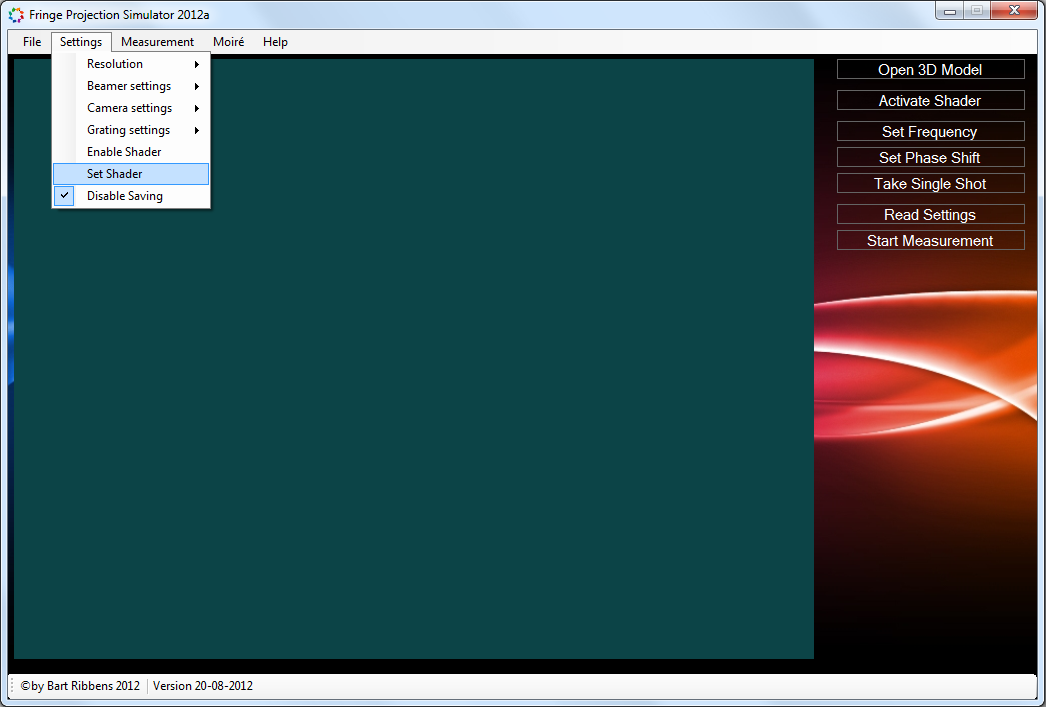
\includegraphics[width=0.85\textwidth, keepaspectratio=true]
	{Graphics/SetShader/setshader.png}
	\caption{Set Shader}
	\label{fig:setshader}
\end{figure}
\subsubsection{Vertex Shader}
\label{sec:VertexShader}
First we choose the vertex shader, which we will be using in this simulation.
\begin{figure}
	\centering
				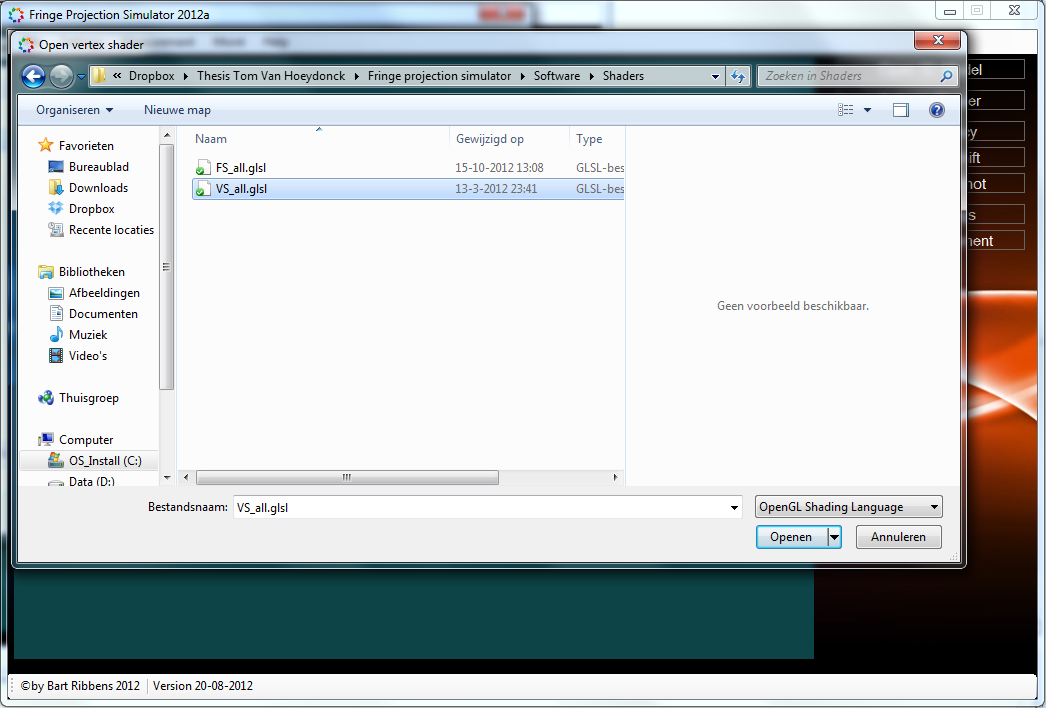
\includegraphics[width=0.85\textwidth, keepaspectratio=true]
	{Graphics/SetShader/vertexshader.png}
	\caption{Vertex Shader}
	\label{fig:vertexshader}
\end{figure}

%%%%%%%%%%%%%%WHAT IS VERTEX SHADER??? MORE INFO%%%%%%%%%%%%%%%%%%%%%%%

Next, we can choose the fragment shader.
\begin{figure}
	\centering
		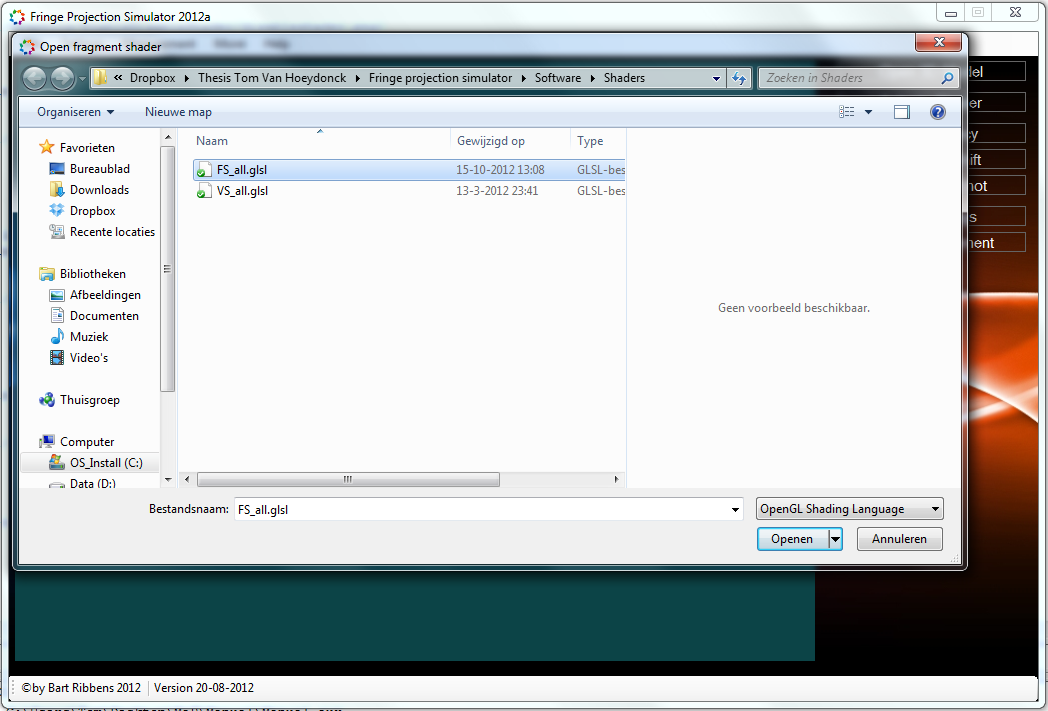
\includegraphics[width=0.85\textwidth, keepaspectratio=true]
	{Graphics/SetShader/fragmentshader.png}
	\caption{Fragment Shader}
	\label{fig:fragmentshader}
\end{figure}

%%%%%%%%%%%%%%%%%%%%%%%%%%%%WHAT IS FRAGMENT SHADER??? MORE INFO%%%%%%%%%%%%%%%%%%%%

\section{Enable/Disable Saving}
\label{sec:EnableDisableSaving}
\begin{figure}
	\centering
			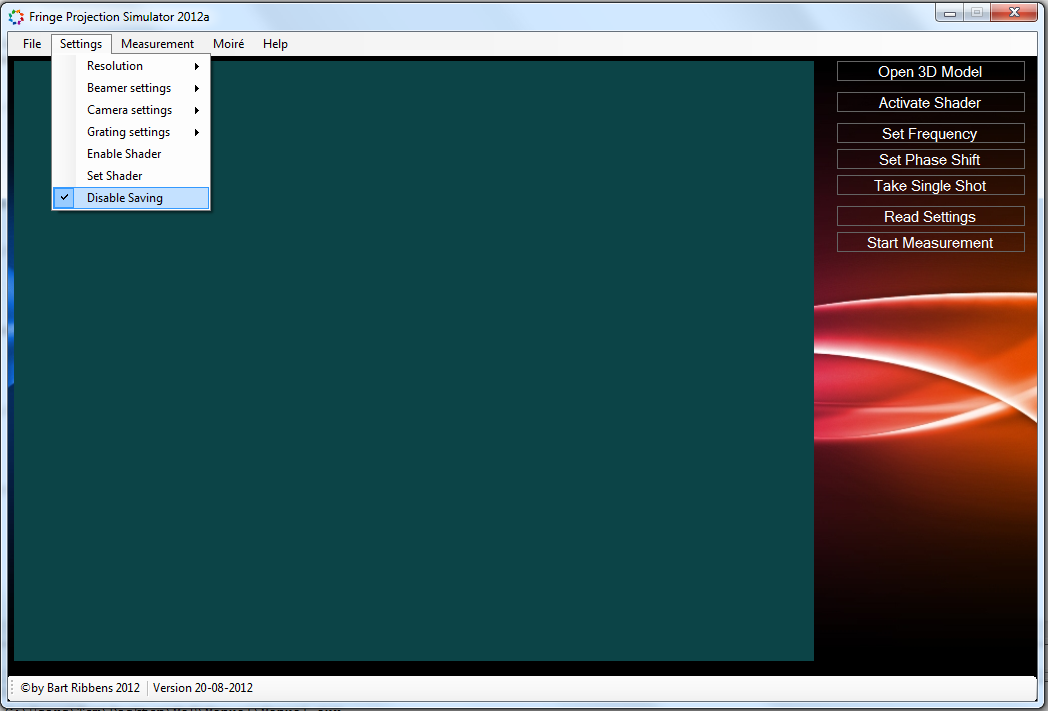
\includegraphics[width=0.85\textwidth, keepaspectratio=true]
	{Graphics/Saving/saving.png}
	\caption{Saving}
	\label{fig:saving}
\end{figure}
When starting up the program, saving is enabled. By clicking this button, you will be unable to save a picture.
If you want to save a picture, simply press the enable save button.
\begin{figure}
	\centering
			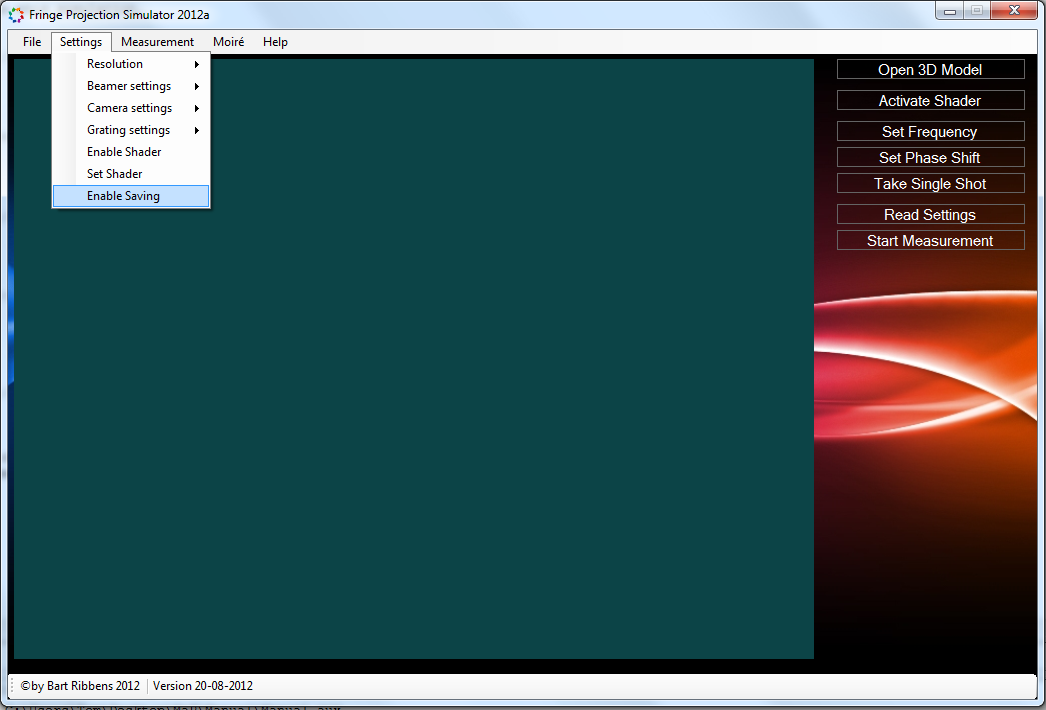
\includegraphics[width=0.85\textwidth, keepaspectratio=true]
	{Graphics/Saving/enablesaving.png}
	\caption{Enable Saving}
	\label{fig:enablesaving}
\end{figure}
\section{Measurement}
\label{sec:Measurement}
With the measurement control, we can change the settings of the pattern that is projected by our beamer.
\begin{figure}
	\centering				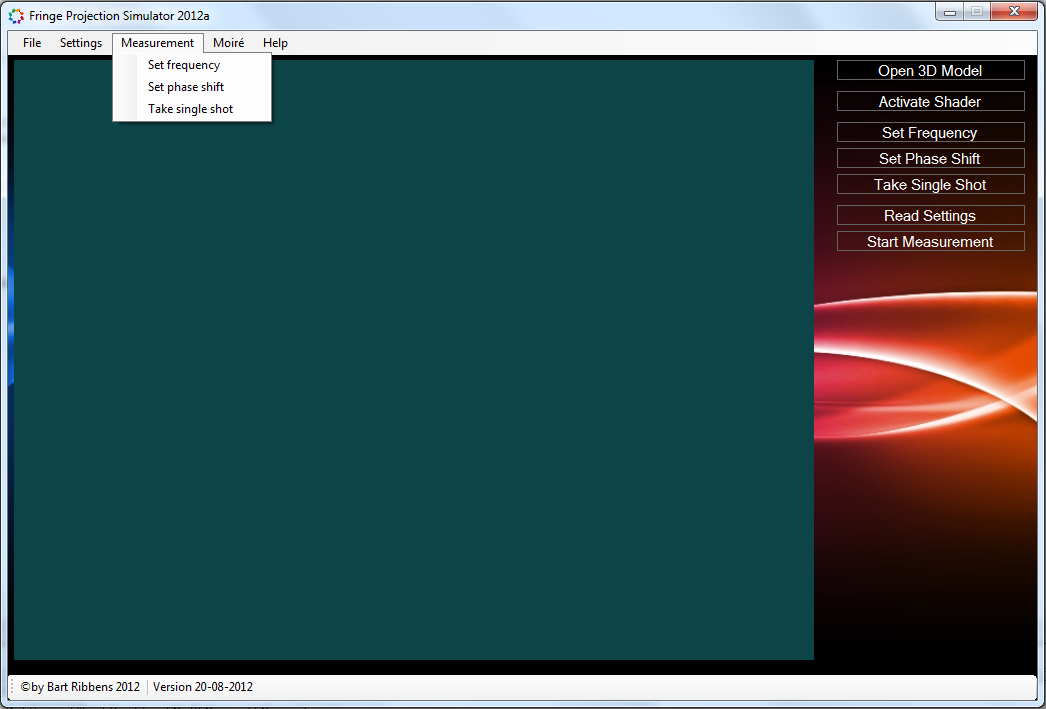
\includegraphics[width=0.85\textwidth, keepaspectratio=true]
	{Graphics/Measurement/measurementsettings.png}
	\caption{Measurement Settings}
	\label{fig:measurementsettings}
\end{figure}
\subsection{Set Frequency}
\label{sec:SetFrequency}
With this control, we can alternate the frequency of the projected pattern.
\begin{figure}
	\centering
				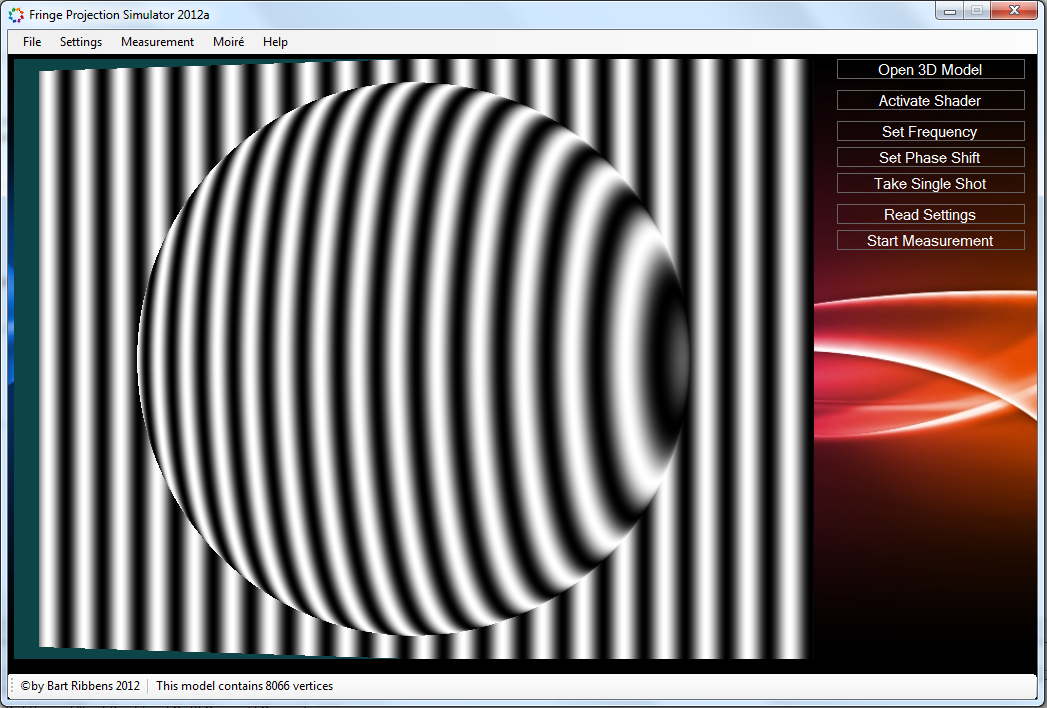
\includegraphics[width=0.85\textwidth, keepaspectratio=true]
	{Graphics/Measurement/20.png}
	\caption{Frequency of 20}
	\label{fig:20}
\end{figure}
In Figure \ref{fig:20}, we can see 20 white lines projected upon the model.
Frequency: 50
\begin{figure}
	\centering
					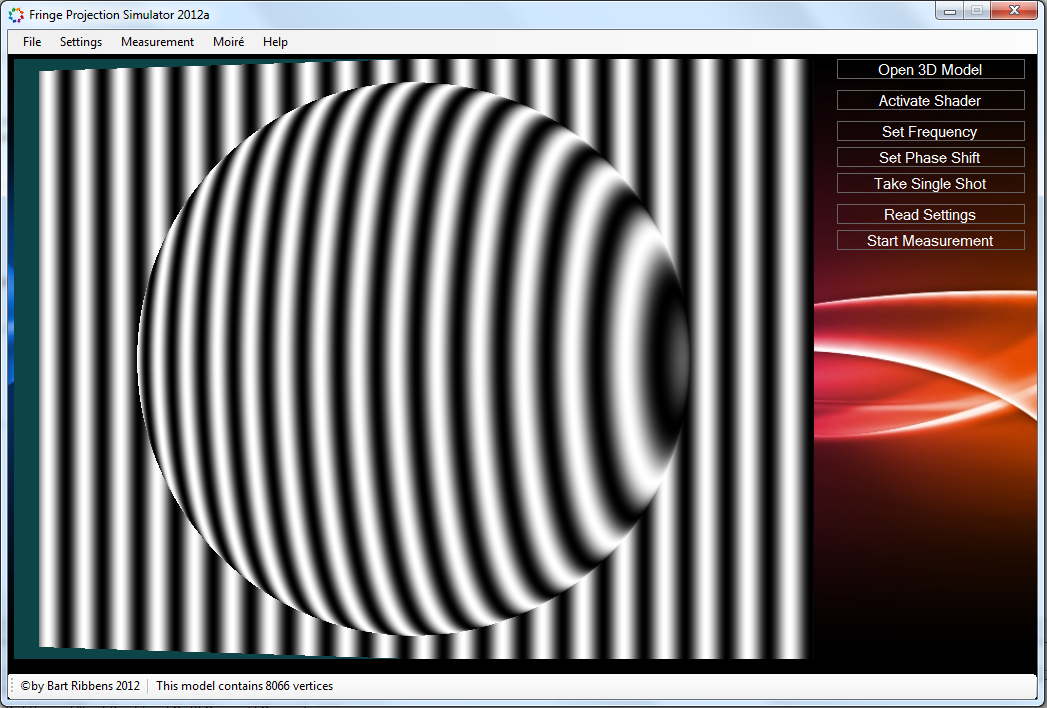
\includegraphics[width=0.85\textwidth, keepaspectratio=true]
	{Graphics/Measurement/20.png}
	\caption{Frequency of 50}
	\label{fig:50}
\end{figure}
When we look at Figure \ref{fig:50}, we see 50 white lines projected onto the model.
\paragraph{Aliasing}
\label{sec:Aliasing}
%Uitleg nodig?
%5http://www.stanford.edu/class/ee368b/Projects/panu/pages/aliasing.html
\begin{figure}
	\centering
	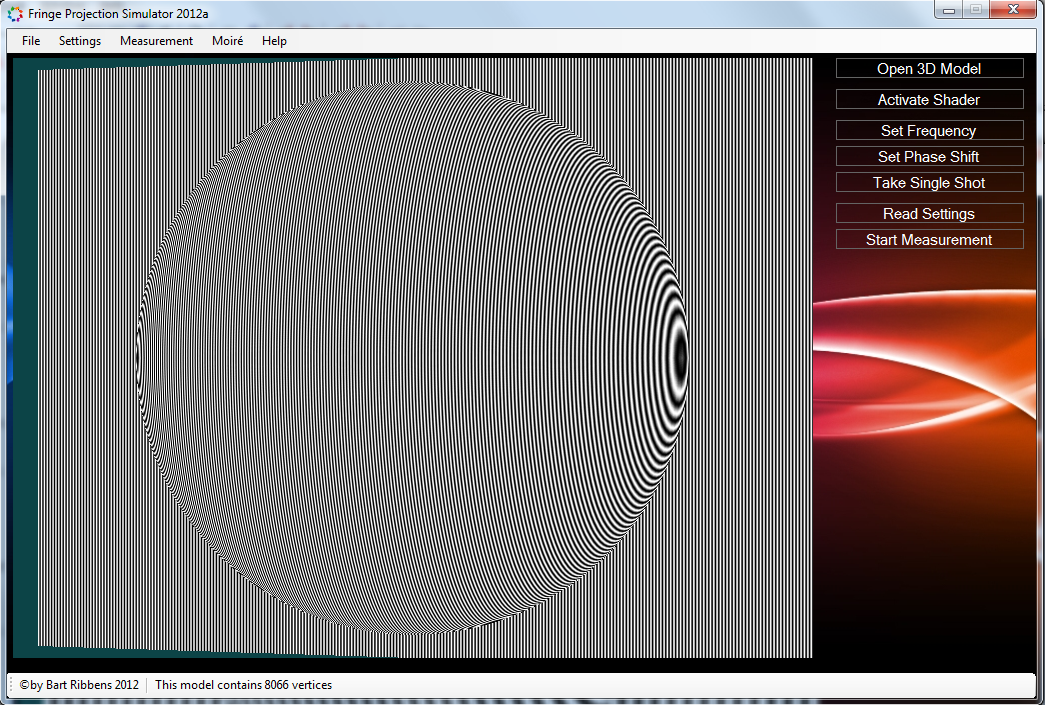
\includegraphics[width=0.85\textwidth, keepaspectratio=true]
	{Graphics/Measurement/250.png}
	\caption{Aliasing}
	\label{fig:250}
\end{figure}
\subsection{Set Phaseshift}
\label{sec:SetPhaseshift}
Phaseshifting is also possible in this simulation.
When clicking this button, a pop up screen will appear.
\begin{figure}
	\centering
					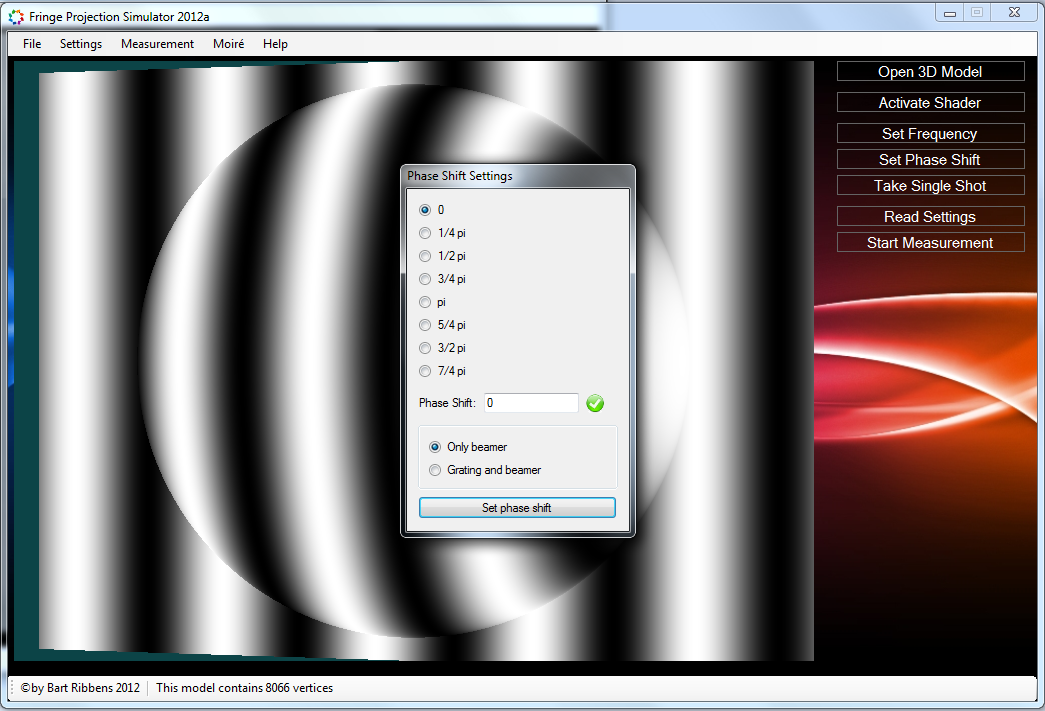
\includegraphics[width=0.85\textwidth, keepaspectratio=true]
	{Graphics/Phaseshift/phaseshift.png}
	\caption{Phaseshift}
	\label{fig:phaseshift}
\end{figure}
Standard the phaseshift is set at 0.
The phaseshift is expressed in radians.
A period is equal to 2PI (360 degrees), this contains one white line and one black line.
When we set the phaseshift at PI/2 radian, we can see that only half the length of the first white line is visible.
\begin{figure}
	\centering
	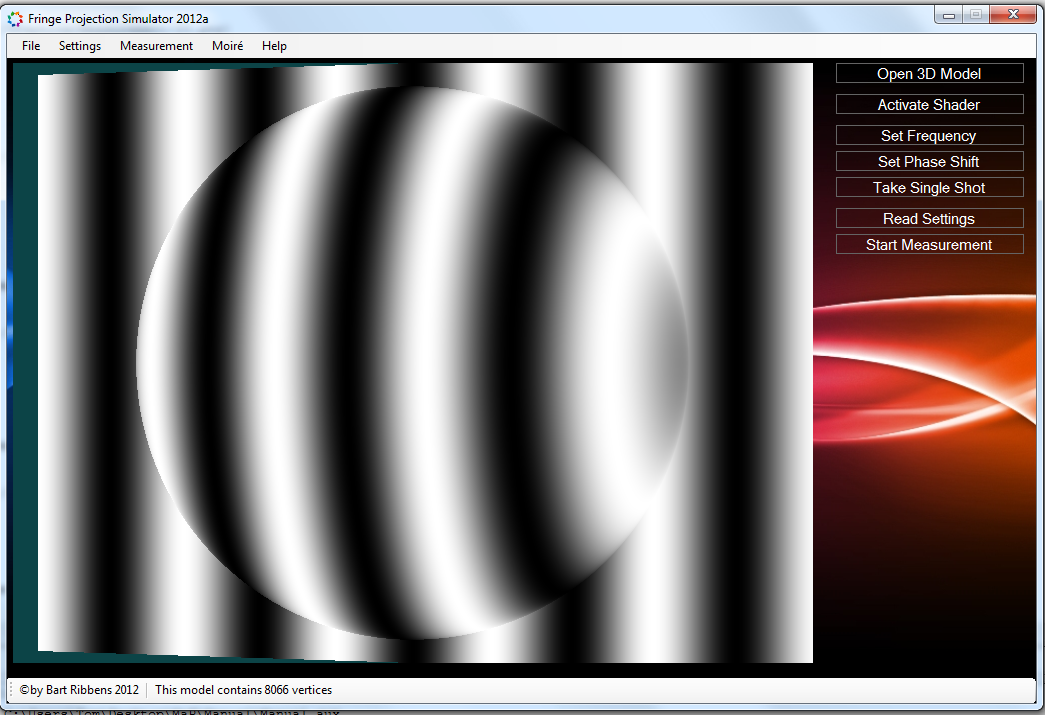
\includegraphics[width=0.85\textwidth, keepaspectratio=true]
	{Graphics/Phaseshift/phaseshiftpi2.png}	
	\caption{Phaseshift PI/2}
	\label{fig:phaseshiftpi2}
\end{figure}
This is because the whole pattern is shifted PI/2 radians (90 degrees), 1/4th of a period.
It is also possible to insert a phaseshift manually.
Instead of only changing the phaseshift of the beamer, we can also set the phaseshift of the beamer and grating together.
\subsection{Take Single Shot}
\label{sec:TakeSingleShot}
By taking a single shot, we can save the file as a .PNG file.
\begin{figure}
	\centering
	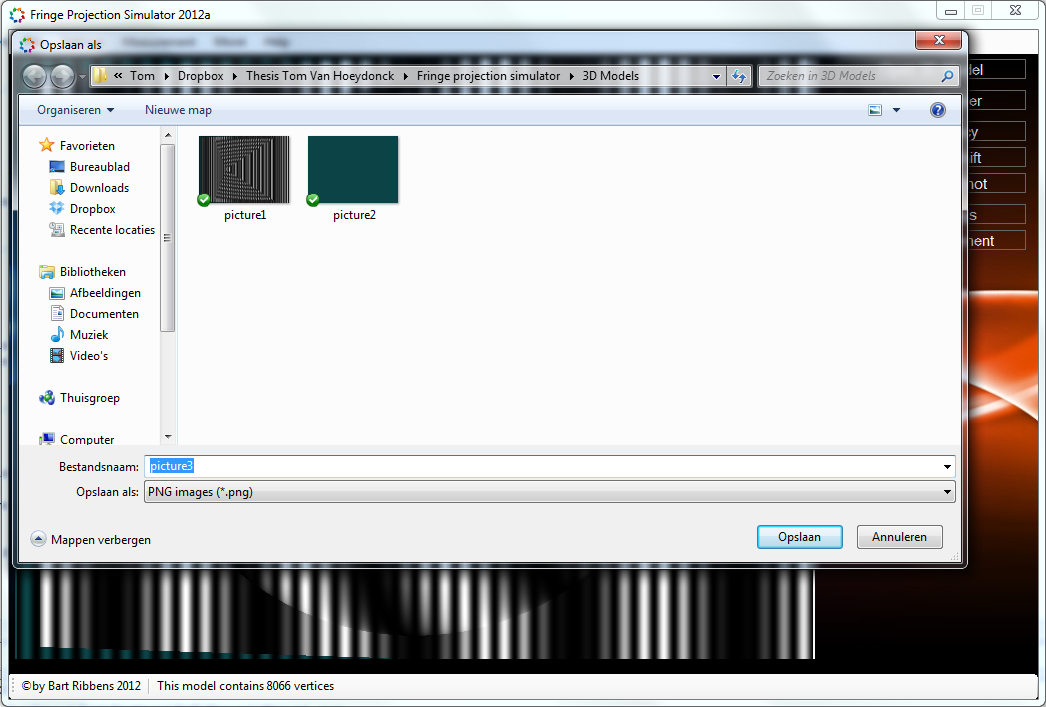
\includegraphics[width=0.85\textwidth, keepaspectratio=true]
	{Graphics/Save/takesingleshot.png}
	\caption{Save File}
	\label{fig:takesingleshot}
\end{figure}
\section{Moir\'e}
In this menu, we can change every aspect of the moir\'e grating.
\begin{figure}
	\centering
	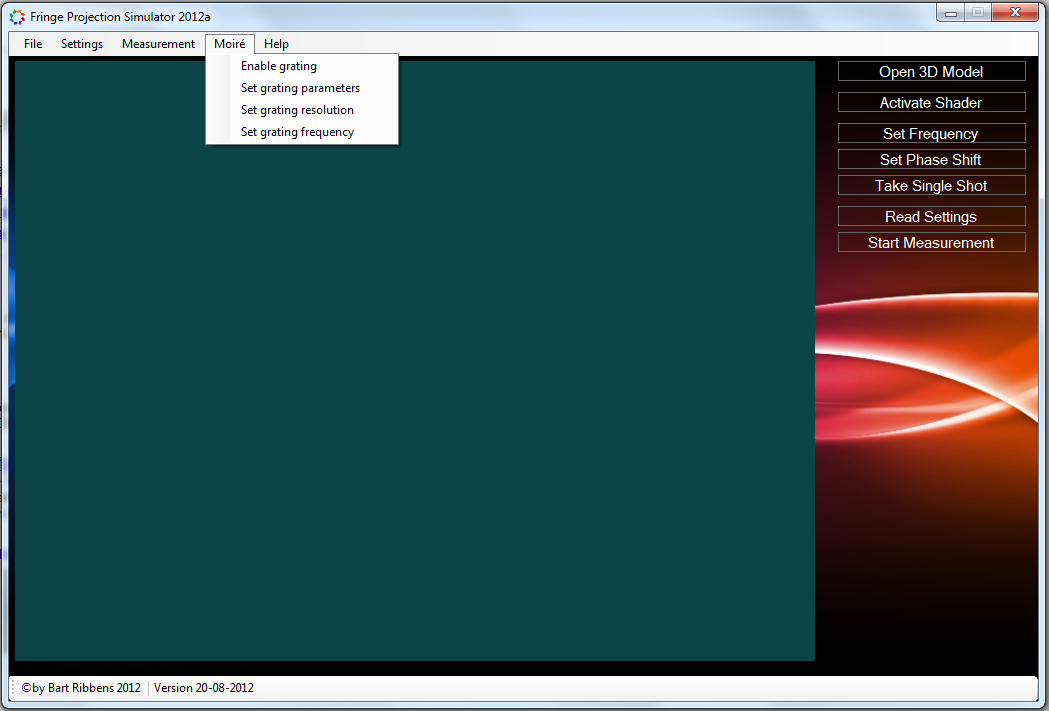
\includegraphics[width=0.85\textwidth, keepaspectratio=true]
	{Graphics/moire/moire.png}
	\caption{Moir\'e}
	\label{fig:Moire}
\end{figure}
\subsection{Enable grating}
Using the enable grating button, allows us to activate the moir\'e grating.
When we start the program and enable the moir\'e grating, it will look like Figure \ref{fig:Moire enabled}.
\begin{figure}
\centering
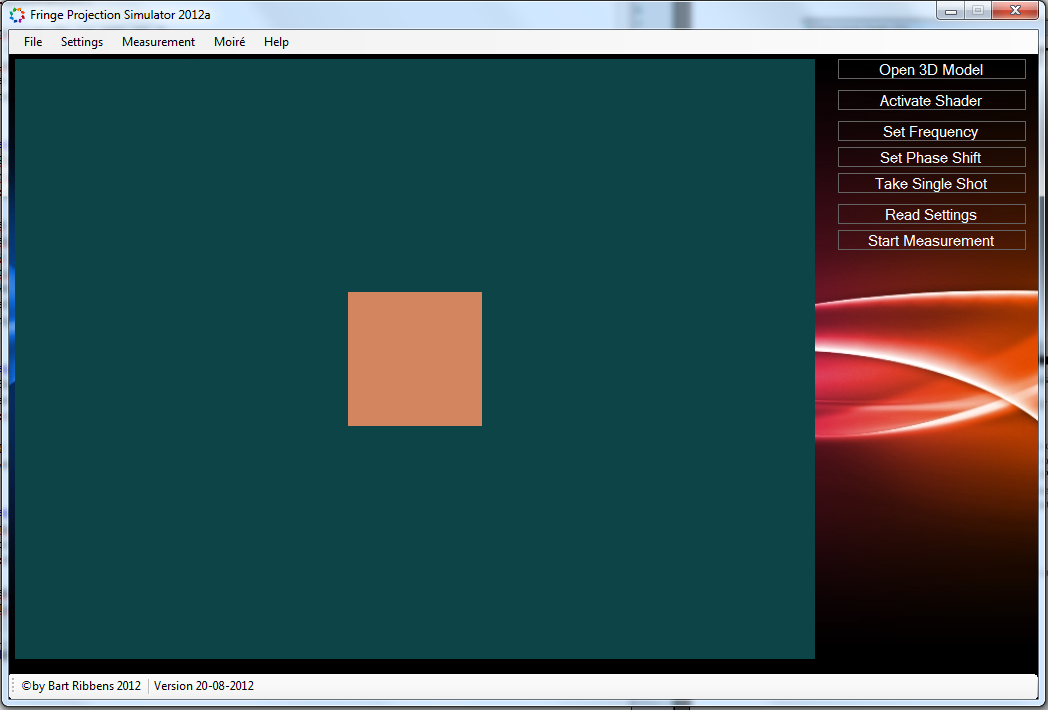
\includegraphics[width=0.85\textwidth, keepaspectratio=true]
	{Graphics/moire/moireenabled.png}
	\caption{Moir\'e enabled}
	\label{fig:Moire enabled}
\end{figure}
We only see a square, but no pattern. This is because we haven't enabled the shader yet.
When we active the shader, we will have a pattern looking like Figure \ref{fig:Moire and shader enabled}.
\begin{figure}
\centering
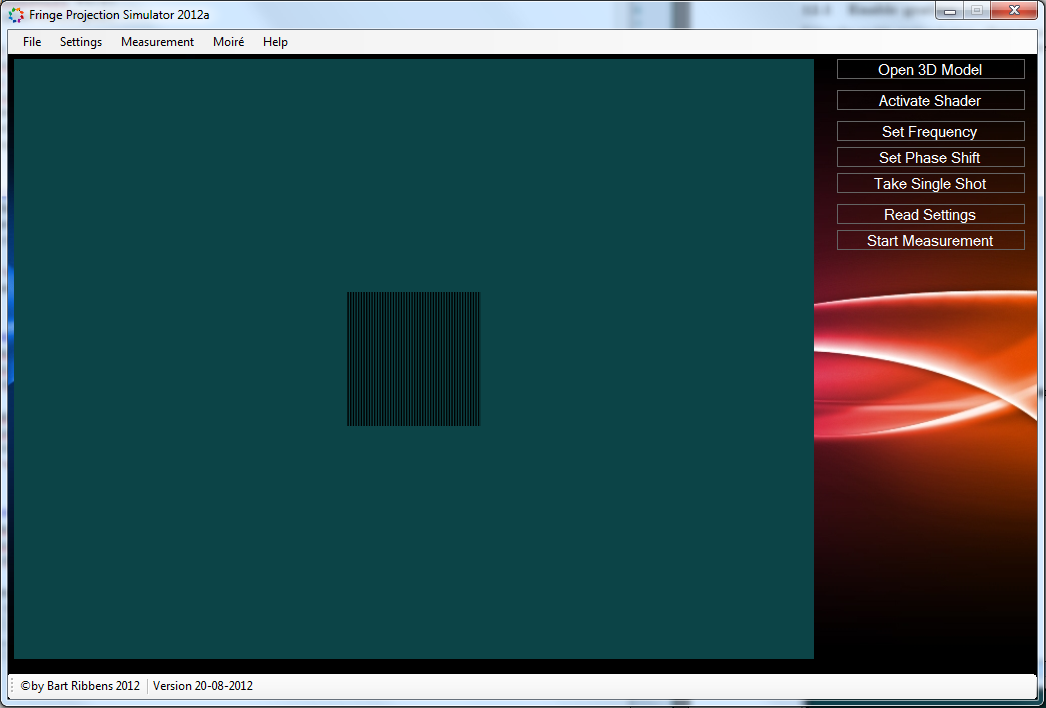
\includegraphics[width=0.85\textwidth, keepaspectratio=true]
	{Graphics/moire/moireenabledandshader.png}
	\caption{Moir\'e and shader enabled}
	\label{fig:Moire and shader enabled}
\end{figure}
In order to get a meaningful output, we still have to adjust the parameters to get a working setup as we will see in our example.
\subparagraph{Set Grating Parameter}
We can choose the position of the grating using this button.
First, we have to insert the X position of our first point.
\begin{figure}
\centering
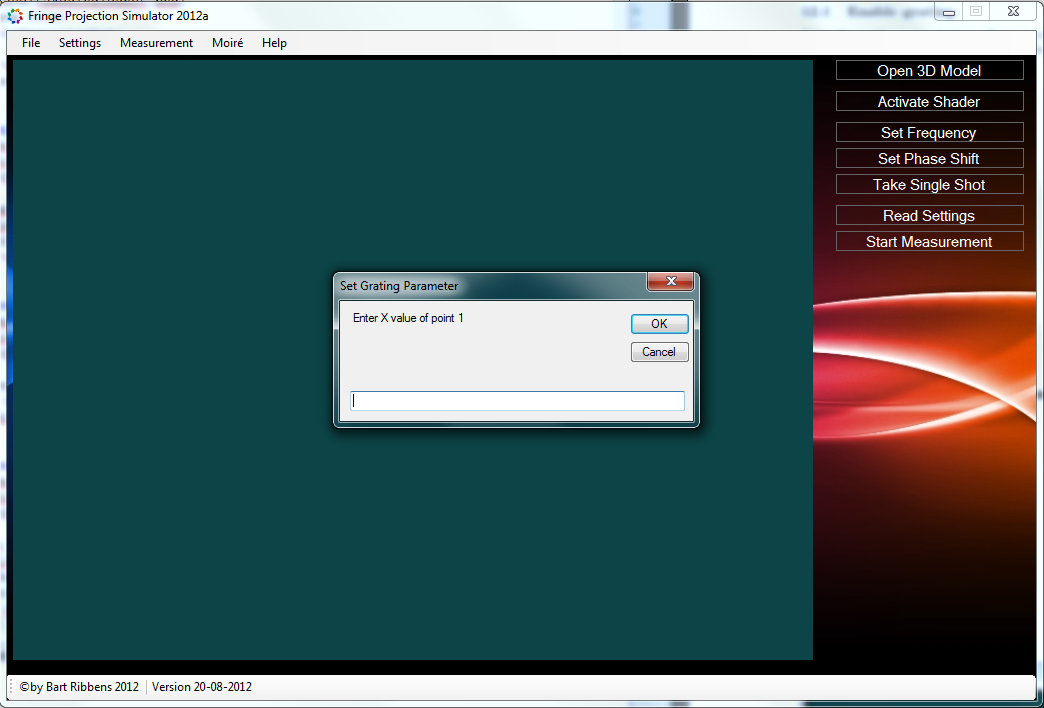
\includegraphics[width=0.85\textwidth, keepaspectratio=true]
	{Graphics/moire/xgrating.png}
	\caption{X position grating}
	\label{fig:X position grating}
\end{figure}
Then we have to enter the Y position and the Z position.
After we inserted our first point, we have to insert the second point.
\begin{figure}
\centering
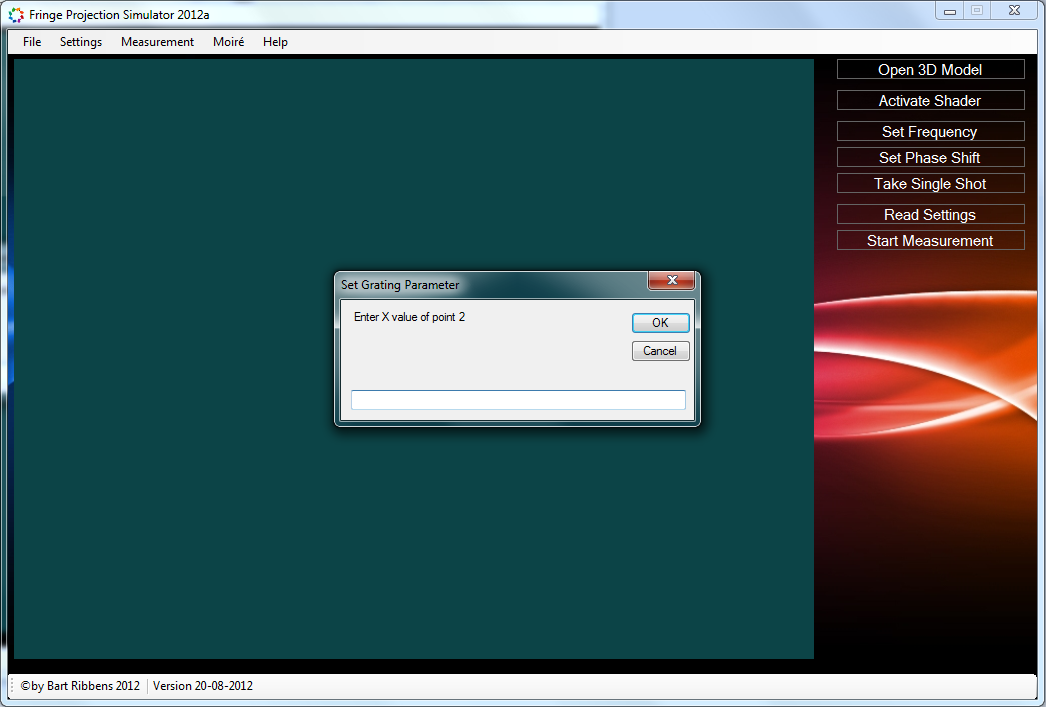
\includegraphics[width=0.85\textwidth, keepaspectratio=true]
	{Graphics/moire/xgrating2.png}
	\caption{X position 2 grating}
	\label{fig:X position 2 grating}
\end{figure}
The first and second point are in order, the bottom left and upper right corners of the grating. This is visualized in Figure \ref{fig:gratings points}.
\begin{figure}
\centering
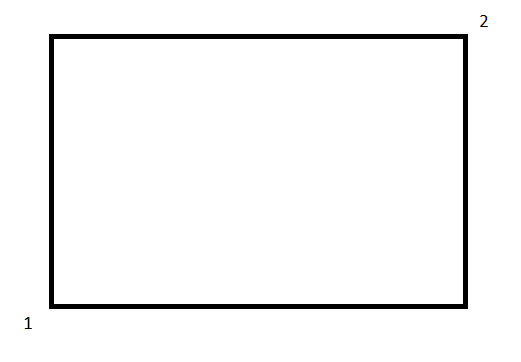
\includegraphics[width=0.85\textwidth, keepaspectratio=true]
	{Graphics/moire/gratingpoints.png}
	\caption{Grating points}
	\label{fig:gratings points}
\end{figure}
\subparagraph{Set Resolution}
By setting the resolution of the grating, we can determine the quality of the display.
When we enter a resolution that is high enough, the quality will be high.
\begin{figure}
\centering
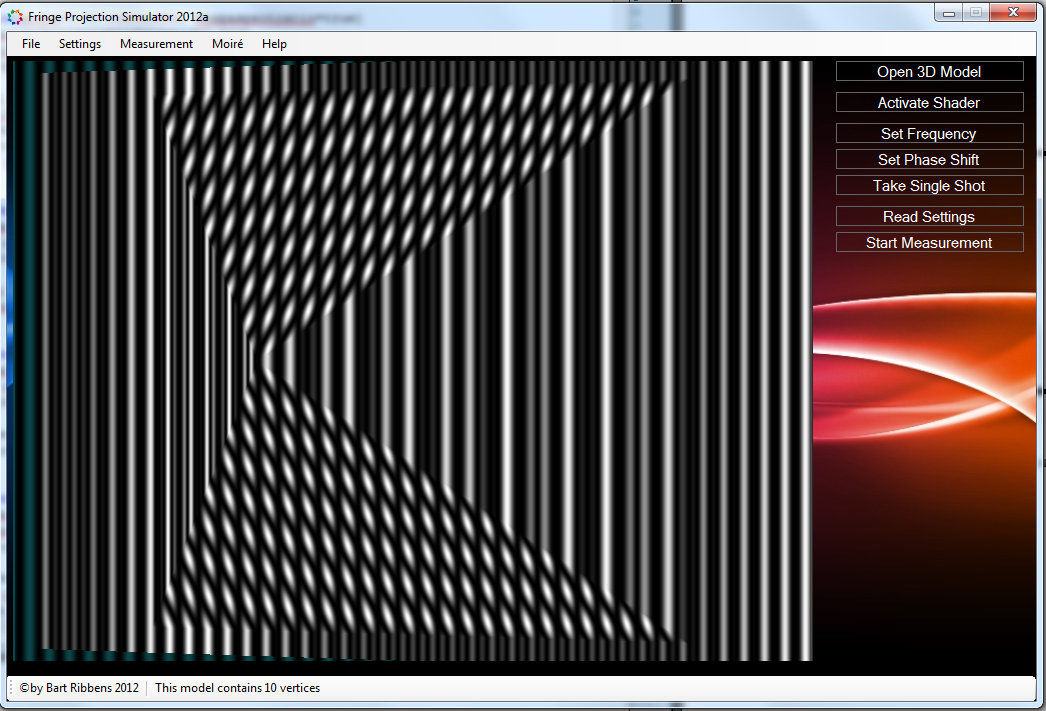
\includegraphics[width=0.85\textwidth, keepaspectratio=true]
	{Graphics/moire/gratingresolution.png}
	\caption{Grating resolution of 20000x20000}
	\label{fig:gratings resolution high}
\end{figure}
Notice that the lines are all smooth.
If we lower the resolution to 500x500, we will notice that the quality is significantly lower than the previous resolution. This effect will occur more when the resolution is lower.
\begin{figure}
\centering
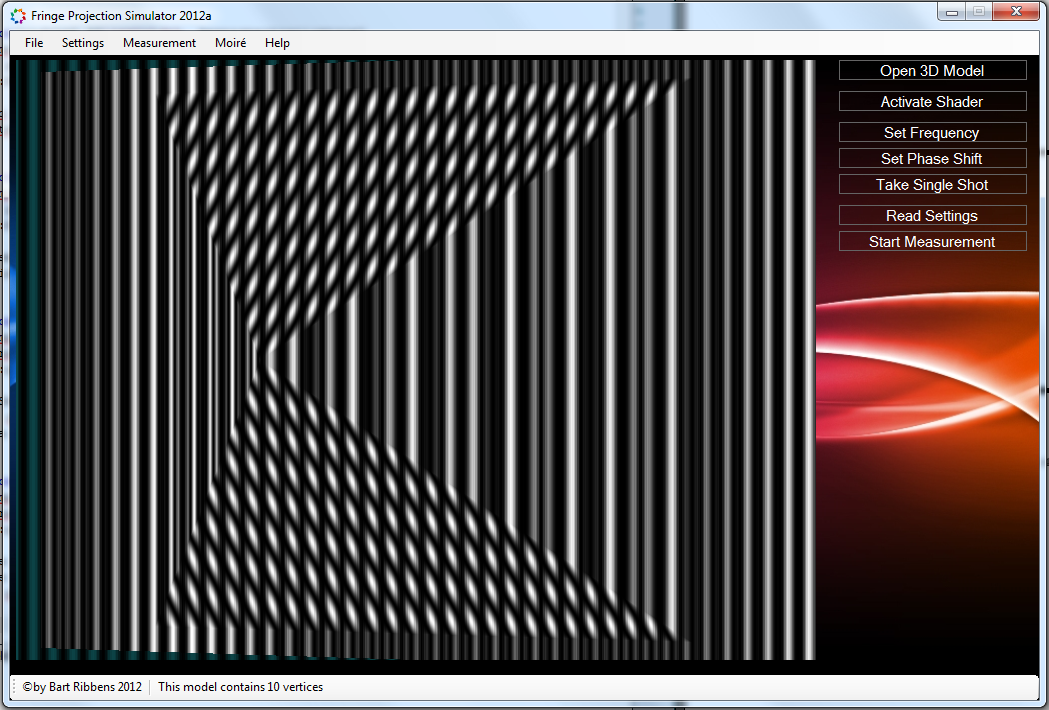
\includegraphics[width=0.85\textwidth, keepaspectratio=true]
	{Graphics/moire/gratingresolutionlow.png}
	\caption{Grating resolution of 500x500}
	\label{fig:gratings resolution low}
\end{figure}
In Figure \ref{fig:gratings resolution low} we notice that there is more fringe in the lines and less smoothness.
\subsection{Set Frequency}
Changing the frequency and phaseshift of the grating can be done with this button.
First we have to enter the frequency of the grating.
\begin{figure}
\centering
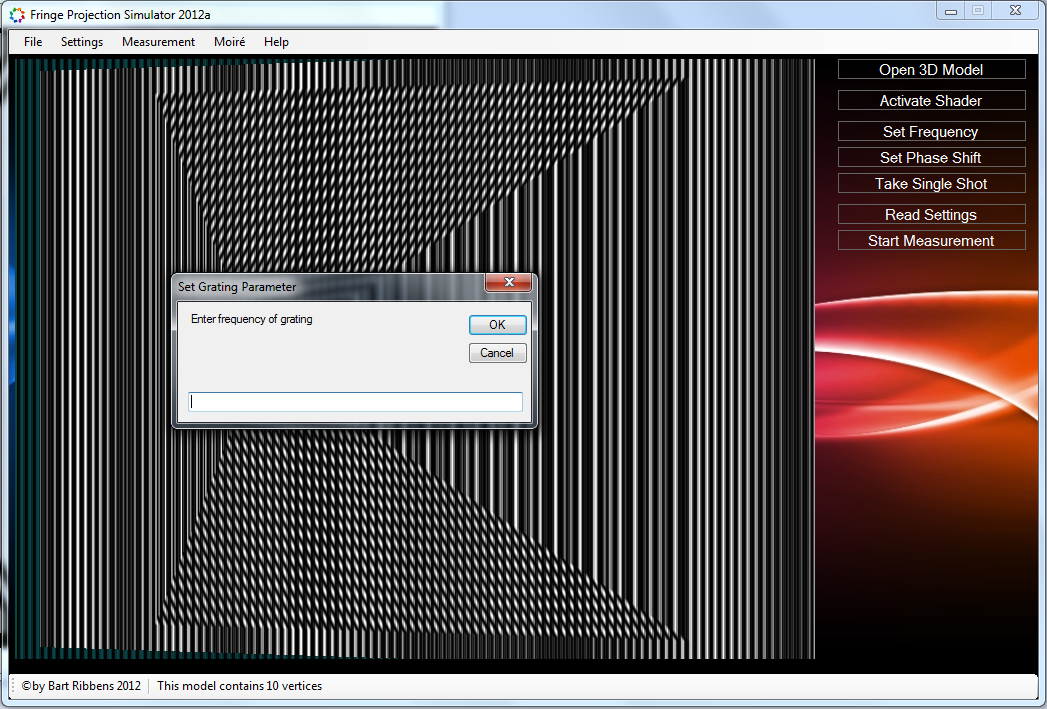
\includegraphics[width=0.85\textwidth, keepaspectratio=true]
	{Graphics/moire/gratingfrequency.png}
	\caption{Grating Frequency}
	\label{fig:grating frequency}
\end{figure}
Next, we can insert the phaseshift of our grating.
\begin{figure}
\centering
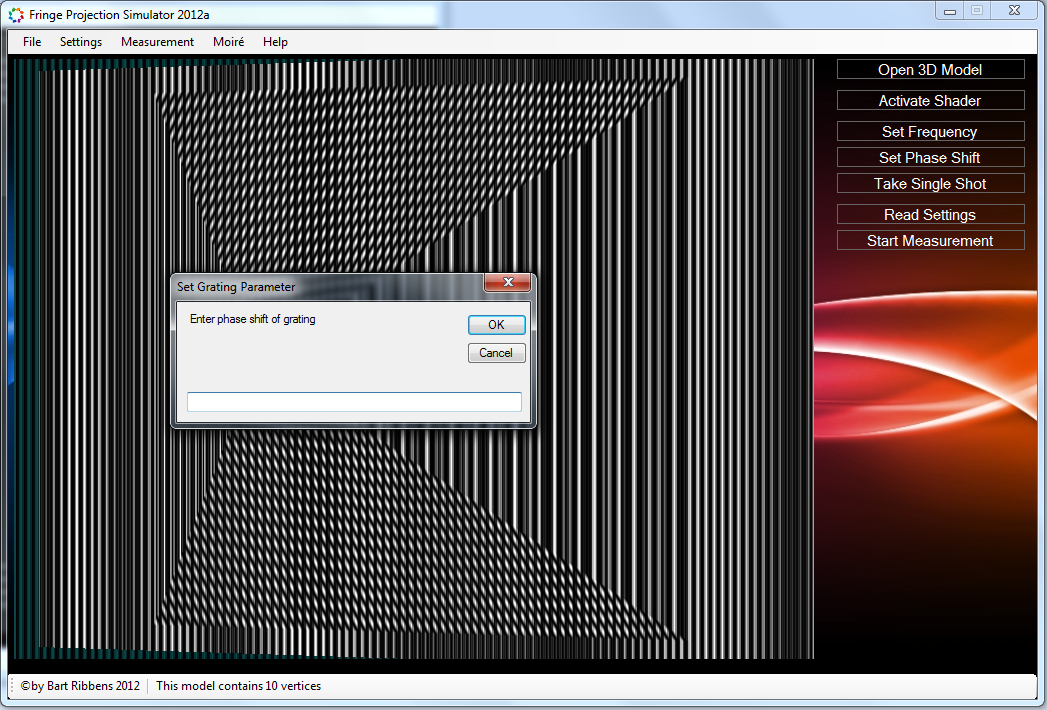
\includegraphics[width=0.85\textwidth, keepaspectratio=true]
	{Graphics/moire/gratingphaseshift.png}
	\caption{Grating Phaseshift}
	\label{fig:grating phaseshift}
\end{figure}
\section{Help}
When there are any questions or remarks, they can be sent using this menu.
\subsection{View Help}
The "View Help" button will sent you to an online contact form as seen in Figure \ref{fig:request form}.
\begin{figure}
\centering
\includegraphics[width=0.85\textwidth, keepaspectratio=true]
	{Graphics/help/request.png}
	\caption{Request Form}
	\label{fig:request form}
\end{figure}
\subsection{About}
More information about the program which is shown in Figure \ref{fig:about}.
\begin{figure}
\centering
\includegraphics[width=0.85\textwidth, keepaspectratio=true]
	{Graphics/help/info.png}
	\caption{About}
	\label{fig:about}
\end{figure}
\part{Button Frame}
These are several buttons which are easily to use for adjusting different parameters.
\section{Open 3D Model}
With this button, we can load a 3D Model within our program. The file has to be of the .STL extension, which means it consists of solely edges. The 3D model contains no volume.
Note that it is possible to create your own 3D Model with inventor and save it as an .STL file, this 3D model can be used in this program.
\section{Activate Shader}
By clicking the activate shader button, we can activate the beamer.
\section{Set Frequency}
Using the Set Frequency button, we can change the frequency of the beamer.
\section{Set Phaseshift}
Changing the phaseshift of the beamer and/or the grating is possible with this button.
\section{Take Single Shot}
When we take a single shot, the image will be saved in a destination path we can choose.
\section{Read Settings}
To make a setup, we can just load the settings containing information about all the parameters into the simulation. This is much faster than manually inserting the parameters every time. These files can be made and edited with notepad.
\begin{figure}
\centering
\includegraphics[width=0.85\textwidth, keepaspectratio=true]
	{Graphics/readsettings/example.png}
	\caption{Example of read settings file}
	\label{fig:read settings}
\end{figure}
\section{Start Measurement}
\label{sec:measurement}
When we want to perform a measurement, we use this button.
The parameters of the measurement are also found in the settings file.
\begin{figure}
\centering
\includegraphics[width=0.85\textwidth, keepaspectratio=true]
	{Graphics/readsettings/measurement.png}
	\caption{Measurement settings}
	\label{fig:measurement settings}
\end{figure}
As we can see in Figure \ref{fig:measurement settings}, the settings of our measurement are present.
\subsection{Mappath}
The destination to which the files will be saved.
\subsection{Filename}
The filename will start with M001, followed by numbers that add up.
\subsection{Blackout}
The number of black screens saved before and after every measurement.
\subsection{Grating Beamer}
The controls "beamer" and "grating" are used to change the parameters of the grating from the beamer.
\subsection{Frequency}
We have a start and a stop frequency, at the beginning of the measurement we will have a frequency of 5. At the end, the frequency will be 30.
\subsection{Phaseshift}
Initially, the phaseshift will be 0. At the end of our measurement, the phaseshift will be 10.
\subsection{Steps}
This control determines in how many steps the change of frequency and phaseshift will occur. In this example, it will be done in 150 steps.
\part{Example of a measurement}
In this part, we will show an example of how a measurement is done and which steps are followed.
\section{Read Settings}
First of all, we have to adjust the parameters of our camera, grating and beamer.
For this example, we will be using the "measurementRef.fpss" file so that all the parameters are already set. Remember that it is possible to edit this file so you don't have to adjust the parameters everytime you restart the program.
\begin{figure}
\centering
\includegraphics[width=0.85\textwidth, keepaspectratio=true]{Graphics/example/readparameters.png}
	\caption{Read parameter settings}
	\label{fig:Read parameter settings}
\end{figure}
After clicking the "Open" button, the display will look as shown in Figure \ref{fig:Plane reference}.
\begin{figure}
\centering
\includegraphics[width=0.85\textwidth, keepaspectratio=true]	{Graphics/example/planereference.png}
	\caption{Plane reference}
	\label{fig:Plane reference}
\end{figure}
We will have a plane reference that we can use for our measurement.
\section{Open 3-D Model}
Next, we will open our 3-D model which we are going to work with.
\begin{figure}
\centering
\includegraphics[width=0.85\textwidth, keepaspectratio=true]	{Graphics/example/open3d.png}
	\caption{Open 3-D model}
	\label{fig:3dmodel}
\end{figure}
As you can see in Figure \ref{fig:3dmodel}, we will be working with a sphere.
Figure \ref{fig:sphere} is what your display should look like after loading the 3-D model.
\begin{figure}
\centering
\includegraphics[width=0.85\textwidth, keepaspectratio=true]	{Graphics/example/open3d.png}
	\caption{Display with sphere}
	\label{fig:sphere}
\end{figure}
\section{Set and activate shader}
We can set the shaders by going to the settings menu, next click on set shader and select the shaders as explained in section \ref{sec:SetShader}. The shaders used in this tutorial are already loaded when starting the program. 
By clicking on activate shader in the button frame, the beamer will be activated.
We will now have a display of our object with the pattern projected onto it as in Figure \ref{fig:sphereandpattern}.
\begin{figure}
\centering
\includegraphics[width=0.85\textwidth, keepaspectratio=true]	{Graphics/example/patroon.png}
	\caption{Display with sphere and pattern}
	\label{fig:sphereandpattern}
\end{figure}
Note that you can adjust the frequency and phaseshift in the measurement menu, but this will have no effect on the measurement that is performed. The only way to adjust the measurement is by changing these settings in the settings file that we opened earlier.
\section{Measurement settings}
You can edit the measurement settings using notepad. After opening the file, you will see all the information that is loaded into the simulation when it is read.
\begin{figure}
\centering
\includegraphics[width=0.85\textwidth, keepaspectratio=true]	{Graphics/example/measurement.png}
	\caption{Measurement settings}
	\label{fig:measurement}
\end{figure}
In Figure \ref{fig:measurement} we see all the information to adjust the measurement.
For more information about these settings, go to section \ref{sec:measurement}.
These settings are standard and can be manually adjusted:
\begin{enumerate}
\item The phaseshift begins at 0 radians and ends at 10 radians.
\item The frequency of our pattern begins at 5 and ends at 30.
\item The measurement will be executed in 150 steps.
\item Before each measurement, there will be 3 black images saved to identify each measurement.
\end{enumerate}
For this example, we will keep the initial value.
\section{Start Measurement}
After clicking the start measurement button, a pop up screen, as shown in Figure \ref{fig:measurementsavingenabled}, will appear indicating that saving is enabled. This is necessary to perform the measurement. Otherwise, the pictures won't be saved.
\begin{figure}
\centering
\includegraphics[width=0.85\textwidth, keepaspectratio=true]	{Graphics/example/measurementsaveenabled.png}
	\caption{Saving enabled}
	\label{fig:measurementsavingenabled}
\end{figure}
During the measurement, you will see the change in frequency and phaseshift.
After the measurement is done, go to the mappath where you saved the file.
\begin{figure}
\centering
\includegraphics[width=0.85\textwidth, keepaspectratio=true]	{Graphics/example/savedimages.png}
	\caption{Images saved within the map}
	\label{fig:savedimages}
\end{figure}
The measurement started with 3 black images and ended with 3 black images. 
In between there are 150 images because the measurement took 150 steps.
If everything went well, it should look like Figure  Figure \ref{fig:savedimages}.
Congratulations, you have succesfully performed a measurement with the Fringe Projection Simulator!
\end{document}